\documentclass[11pt]{article}
\usepackage[textwidth=18.0cm, textheight=23.0cm, top=2.0cm]{geometry}
\usepackage{pst-all}
\usepackage{amssymb}
\usepackage{tikz}
\usepackage{underscore}\begin{document}
\pagestyle{empty}


ClassName: \underline{\textbf{Class_05.2bp-35}}
\par
BinSize: \underline{\textbf{100 × 100}}
\par
ReduceSize: \underline{\textbf{100 × 100}}
\par
TypeNum: \underline{\textbf{80}}
\par
Num: \underline{\textbf{80}}
\par
OutS: \underline{\textbf{260000}}
\par
InS: \underline{\textbf{215710}}
\par
Rate: \underline{\textbf{0.830}}
\par
UB: \underline{\textbf{26}}
\par
LB0: \underline{\textbf{25}}
\par
LB: \underline{\textbf{26}}
\par
LBWithCut: \underline{\textbf{26}}
\par
NodeCut: \underline{\textbf{0}}
\par
ExtendedNodeCnt: \underline{\textbf{1}}
\par
GenNodeCnt: \underline{\textbf{1}}
\par
PrimalNode: \underline{\textbf{0}}
\par
ColumnCount: \underline{\textbf{74}}
\par
TotalCutCount: \underline{\textbf{0}}
\par
RootCutCount: \underline{\textbf{0}}
\par
LPSolverCnt: \underline{\textbf{49}}
\par
PricingSolverCnt: \underline{\textbf{49}}
\par
BranchAndBoundNum: \underline{\textbf{1}}
\par
isOpt: \underline{\textbf{true}}
\par
TimeOnPrimal: \underline{\textbf{0.000 s}}
\par
TimeOnPricing: \underline{\textbf{3.064 s}}
\par
TimeOnRmp: \underline{\textbf{0.062 s}}
\par
TotalTime: \underline{\textbf{3.220 s}}
\par
\newpage


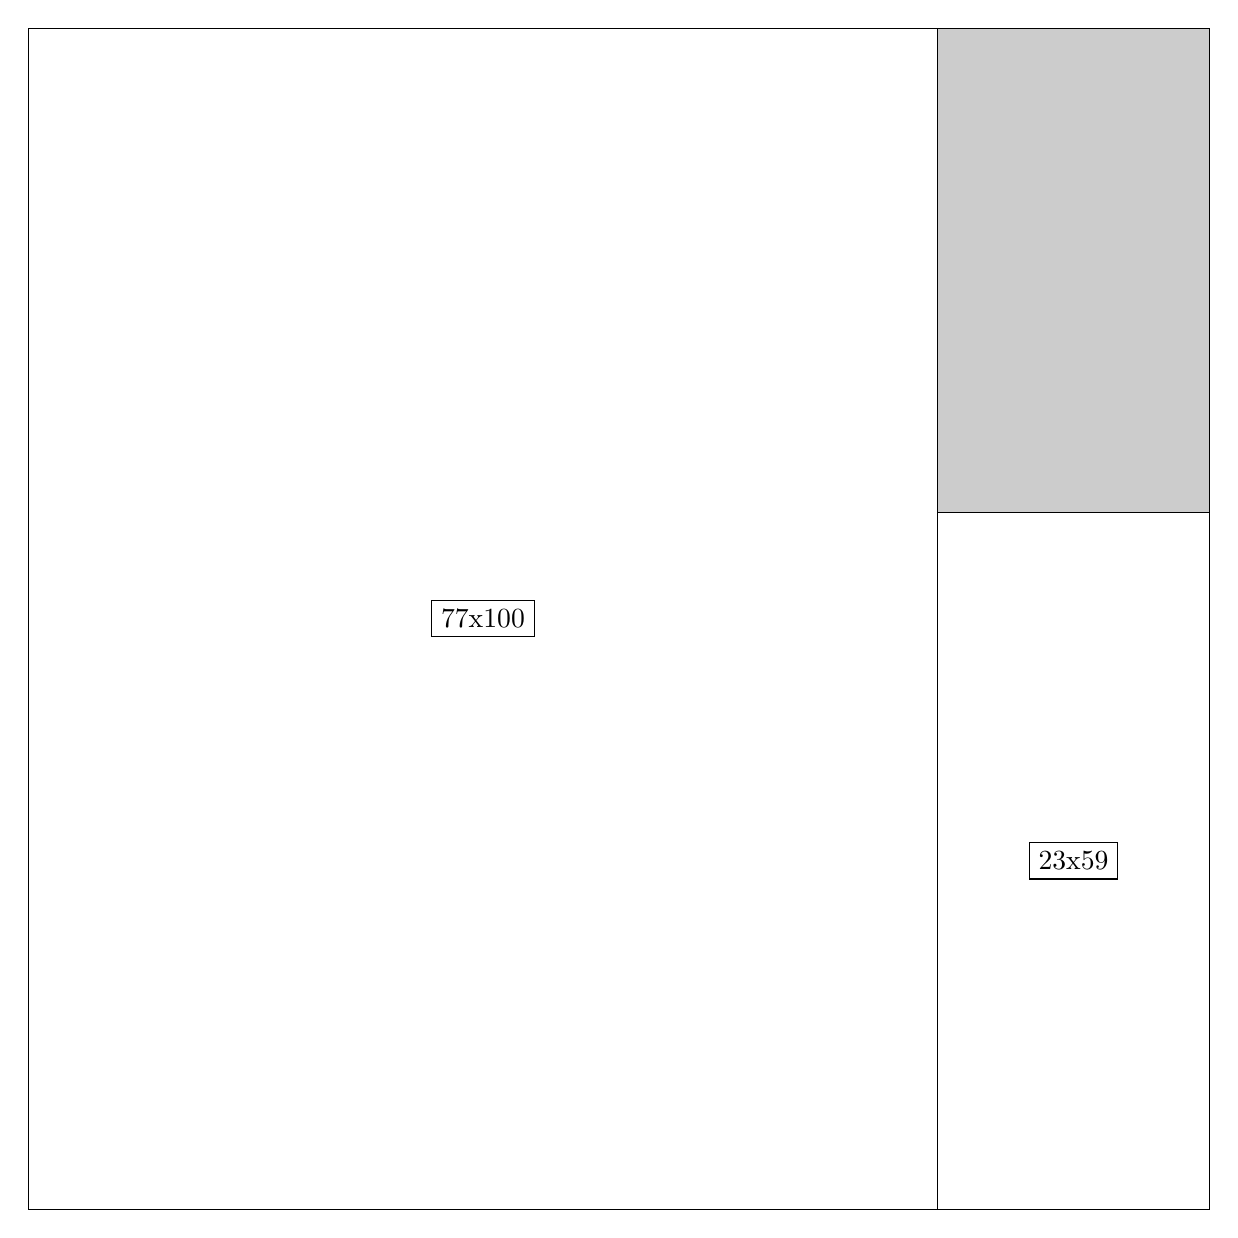
\begin{tikzpicture}[shorten >=1pt,scale=1.0,every node/.style={scale=1.0},->]
\tikzstyle{vertex}=[circle,fill=black!25,minimum size=14pt,inner sep=0pt]
\filldraw[fill=gray!40!white, draw=black] (0,0) rectangle (15.0,15.0);
\foreach \name/\x/\y/\w/\h in {77x100/0.0/0.0/11.549999999999999/15.0,23x59/11.549999999999999/0.0/3.4499999999999997/8.85}
\filldraw[fill=white!40!white, draw=black] (\x,\y) rectangle node[draw] (\name) {\name} ++(\w,\h);
\end{tikzpicture}


w =77 , h =100 , x =0 , y =0 , v =7700
\par
w =23 , h =59 , x =77 , y =0 , v =1357
\par
\newpage


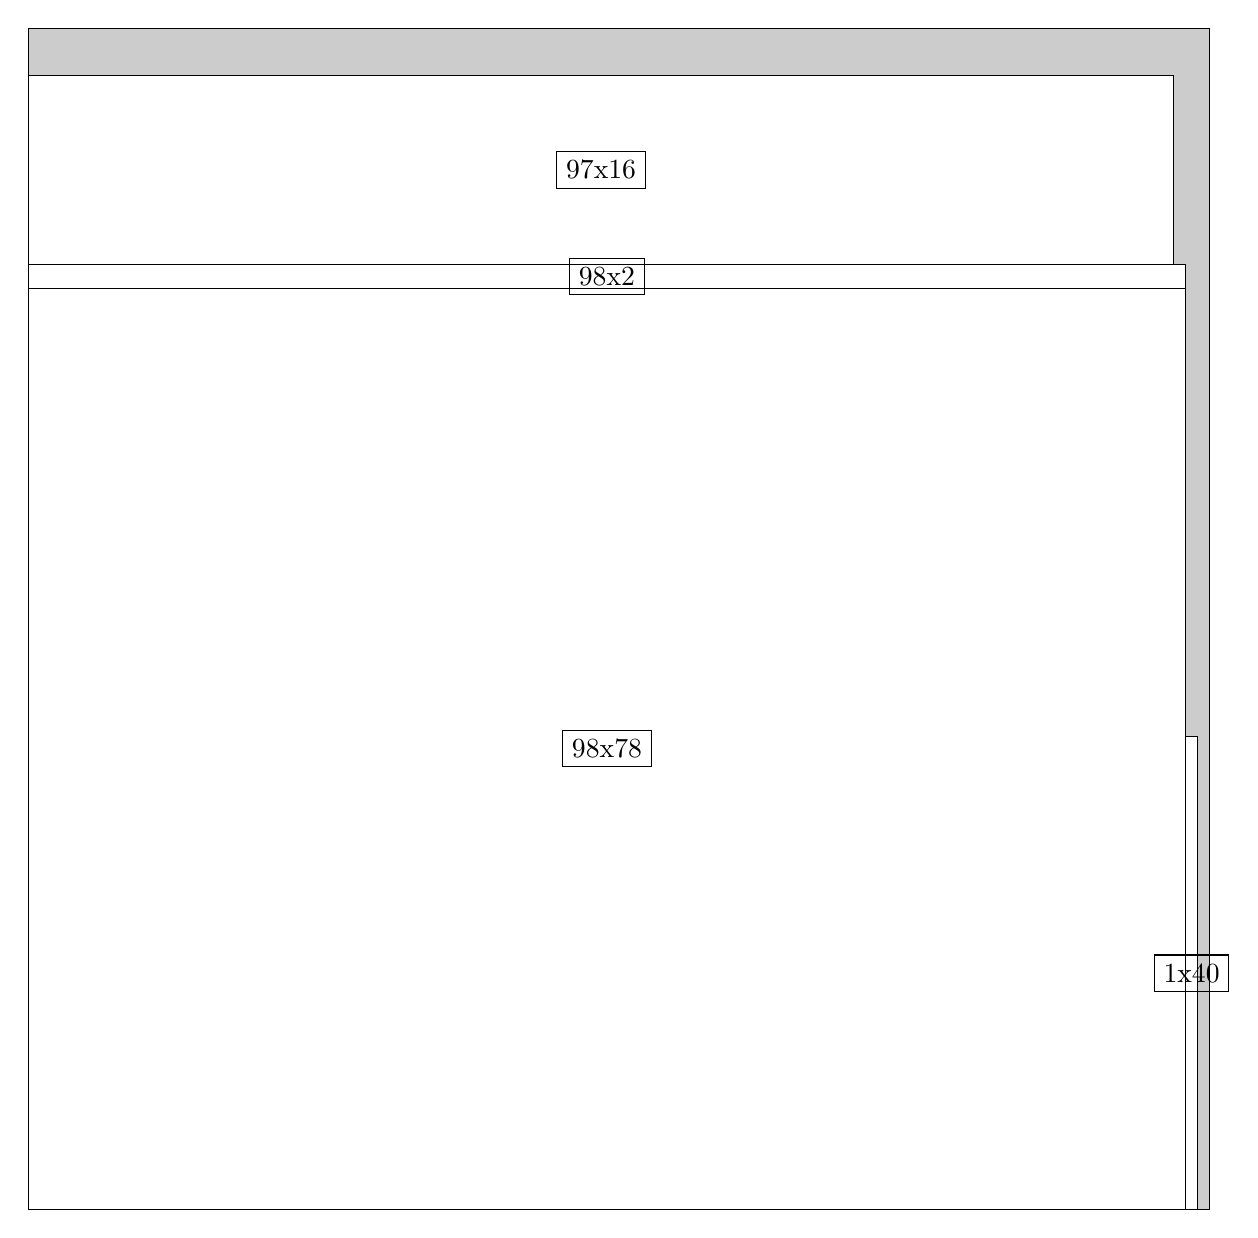
\begin{tikzpicture}[shorten >=1pt,scale=1.0,every node/.style={scale=1.0},->]
\tikzstyle{vertex}=[circle,fill=black!25,minimum size=14pt,inner sep=0pt]
\filldraw[fill=gray!40!white, draw=black] (0,0) rectangle (15.0,15.0);
\foreach \name/\x/\y/\w/\h in {98x78/0.0/0.0/14.7/11.7,97x16/0.0/12.0/14.549999999999999/2.4,98x2/0.0/11.7/14.7/0.3,1x40/14.7/0.0/0.15/6.0}
\filldraw[fill=white!40!white, draw=black] (\x,\y) rectangle node[draw] (\name) {\name} ++(\w,\h);
\end{tikzpicture}


w =98 , h =78 , x =0 , y =0 , v =7644
\par
w =97 , h =16 , x =0 , y =80 , v =1552
\par
w =98 , h =2 , x =0 , y =78 , v =196
\par
w =1 , h =40 , x =98 , y =0 , v =40
\par
\newpage


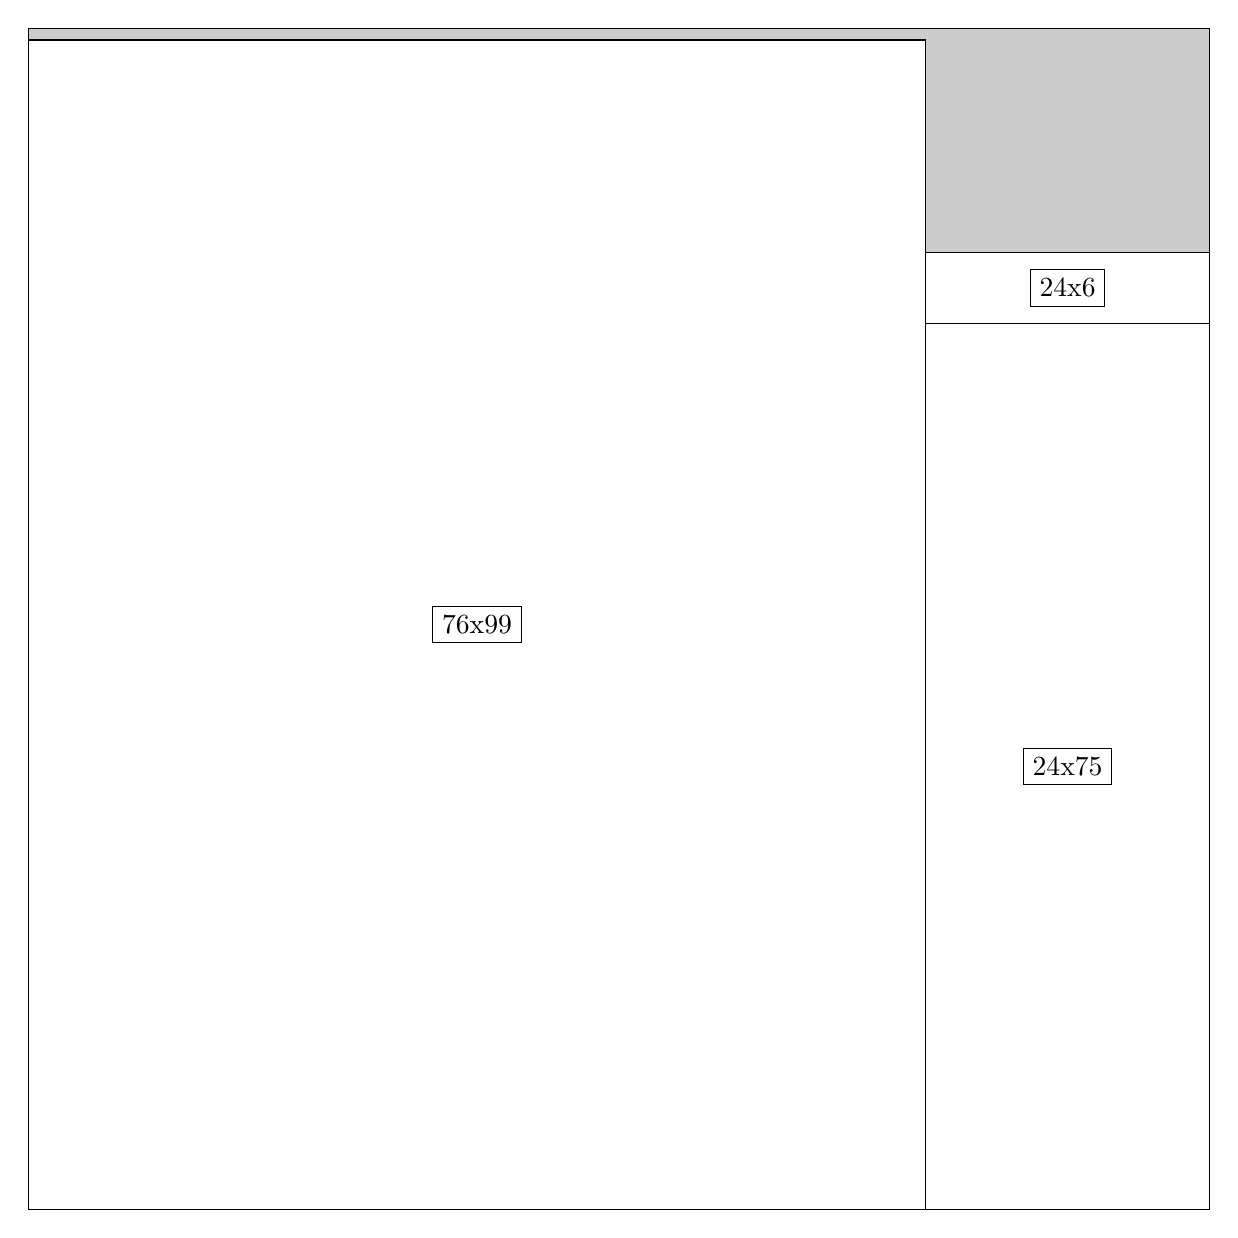
\begin{tikzpicture}[shorten >=1pt,scale=1.0,every node/.style={scale=1.0},->]
\tikzstyle{vertex}=[circle,fill=black!25,minimum size=14pt,inner sep=0pt]
\filldraw[fill=gray!40!white, draw=black] (0,0) rectangle (15.0,15.0);
\foreach \name/\x/\y/\w/\h in {76x99/0.0/0.0/11.4/14.85,24x75/11.4/0.0/3.5999999999999996/11.25,24x6/11.4/11.25/3.5999999999999996/0.8999999999999999}
\filldraw[fill=white!40!white, draw=black] (\x,\y) rectangle node[draw] (\name) {\name} ++(\w,\h);
\end{tikzpicture}


w =76 , h =99 , x =0 , y =0 , v =7524
\par
w =24 , h =75 , x =76 , y =0 , v =1800
\par
w =24 , h =6 , x =76 , y =75 , v =144
\par
\newpage


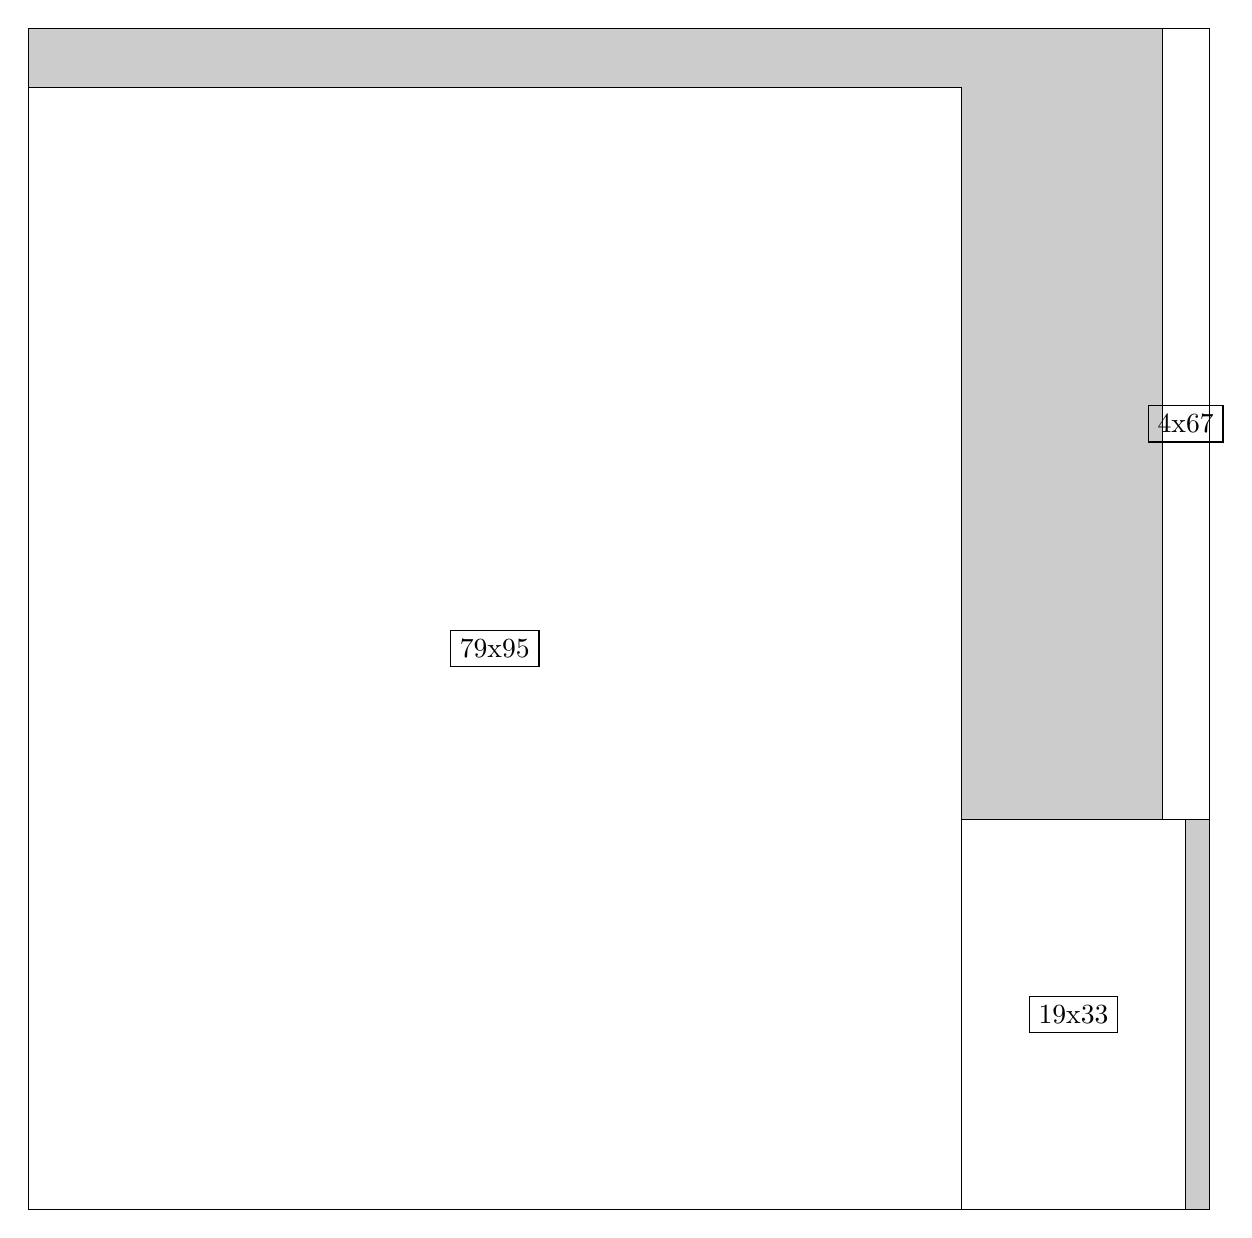
\begin{tikzpicture}[shorten >=1pt,scale=1.0,every node/.style={scale=1.0},->]
\tikzstyle{vertex}=[circle,fill=black!25,minimum size=14pt,inner sep=0pt]
\filldraw[fill=gray!40!white, draw=black] (0,0) rectangle (15.0,15.0);
\foreach \name/\x/\y/\w/\h in {79x95/0.0/0.0/11.85/14.25,19x33/11.85/0.0/2.85/4.95,4x67/14.399999999999999/4.95/0.6/10.049999999999999}
\filldraw[fill=white!40!white, draw=black] (\x,\y) rectangle node[draw] (\name) {\name} ++(\w,\h);
\end{tikzpicture}


w =79 , h =95 , x =0 , y =0 , v =7505
\par
w =19 , h =33 , x =79 , y =0 , v =627
\par
w =4 , h =67 , x =96 , y =33 , v =268
\par
\newpage


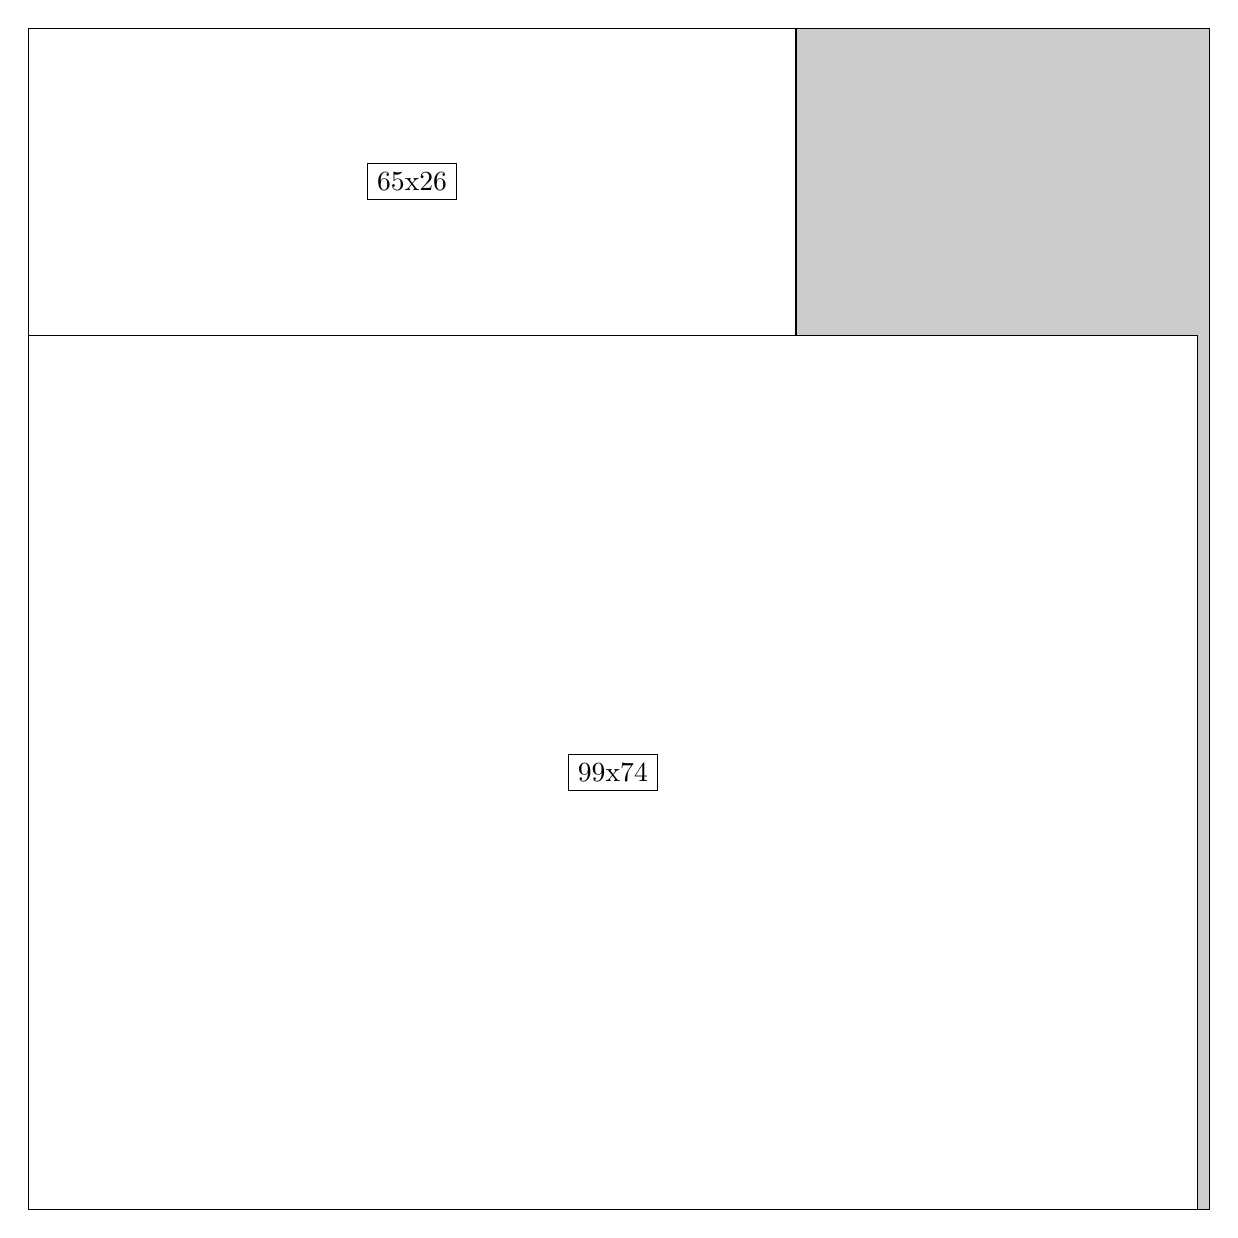
\begin{tikzpicture}[shorten >=1pt,scale=1.0,every node/.style={scale=1.0},->]
\tikzstyle{vertex}=[circle,fill=black!25,minimum size=14pt,inner sep=0pt]
\filldraw[fill=gray!40!white, draw=black] (0,0) rectangle (15.0,15.0);
\foreach \name/\x/\y/\w/\h in {99x74/0.0/0.0/14.85/11.1,65x26/0.0/11.1/9.75/3.9}
\filldraw[fill=white!40!white, draw=black] (\x,\y) rectangle node[draw] (\name) {\name} ++(\w,\h);
\end{tikzpicture}


w =99 , h =74 , x =0 , y =0 , v =7326
\par
w =65 , h =26 , x =0 , y =74 , v =1690
\par
\newpage


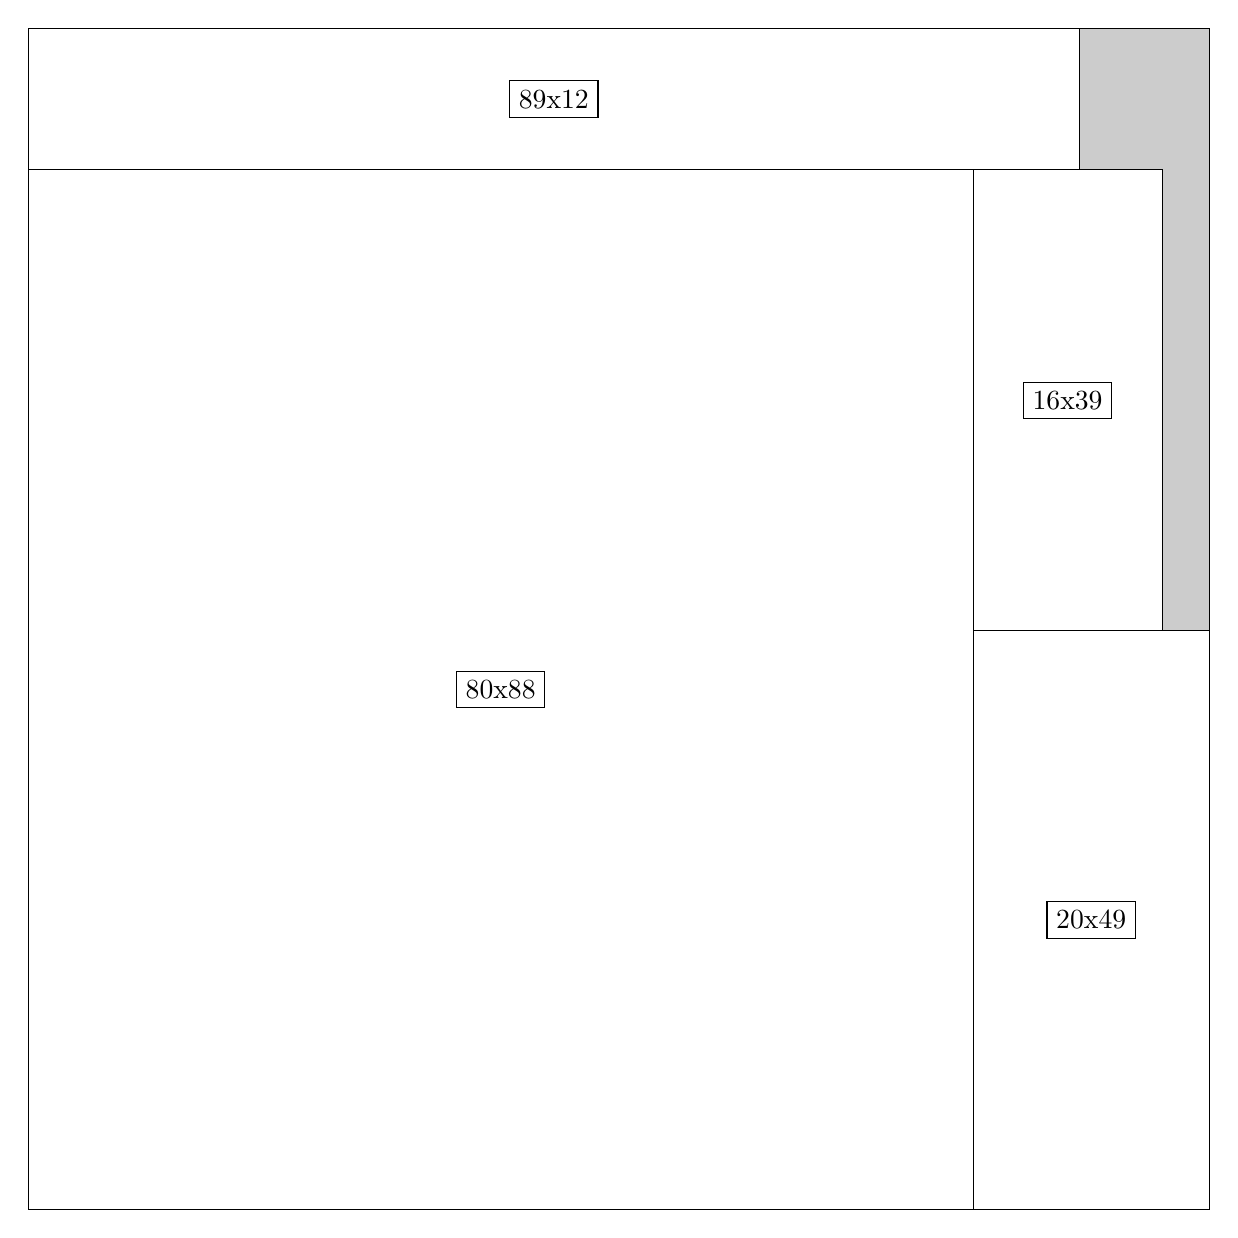
\begin{tikzpicture}[shorten >=1pt,scale=1.0,every node/.style={scale=1.0},->]
\tikzstyle{vertex}=[circle,fill=black!25,minimum size=14pt,inner sep=0pt]
\filldraw[fill=gray!40!white, draw=black] (0,0) rectangle (15.0,15.0);
\foreach \name/\x/\y/\w/\h in {80x88/0.0/0.0/12.0/13.2,89x12/0.0/13.2/13.35/1.7999999999999998,20x49/12.0/0.0/3.0/7.35,16x39/12.0/7.35/2.4/5.85}
\filldraw[fill=white!40!white, draw=black] (\x,\y) rectangle node[draw] (\name) {\name} ++(\w,\h);
\end{tikzpicture}


w =80 , h =88 , x =0 , y =0 , v =7040
\par
w =89 , h =12 , x =0 , y =88 , v =1068
\par
w =20 , h =49 , x =80 , y =0 , v =980
\par
w =16 , h =39 , x =80 , y =49 , v =624
\par
\newpage


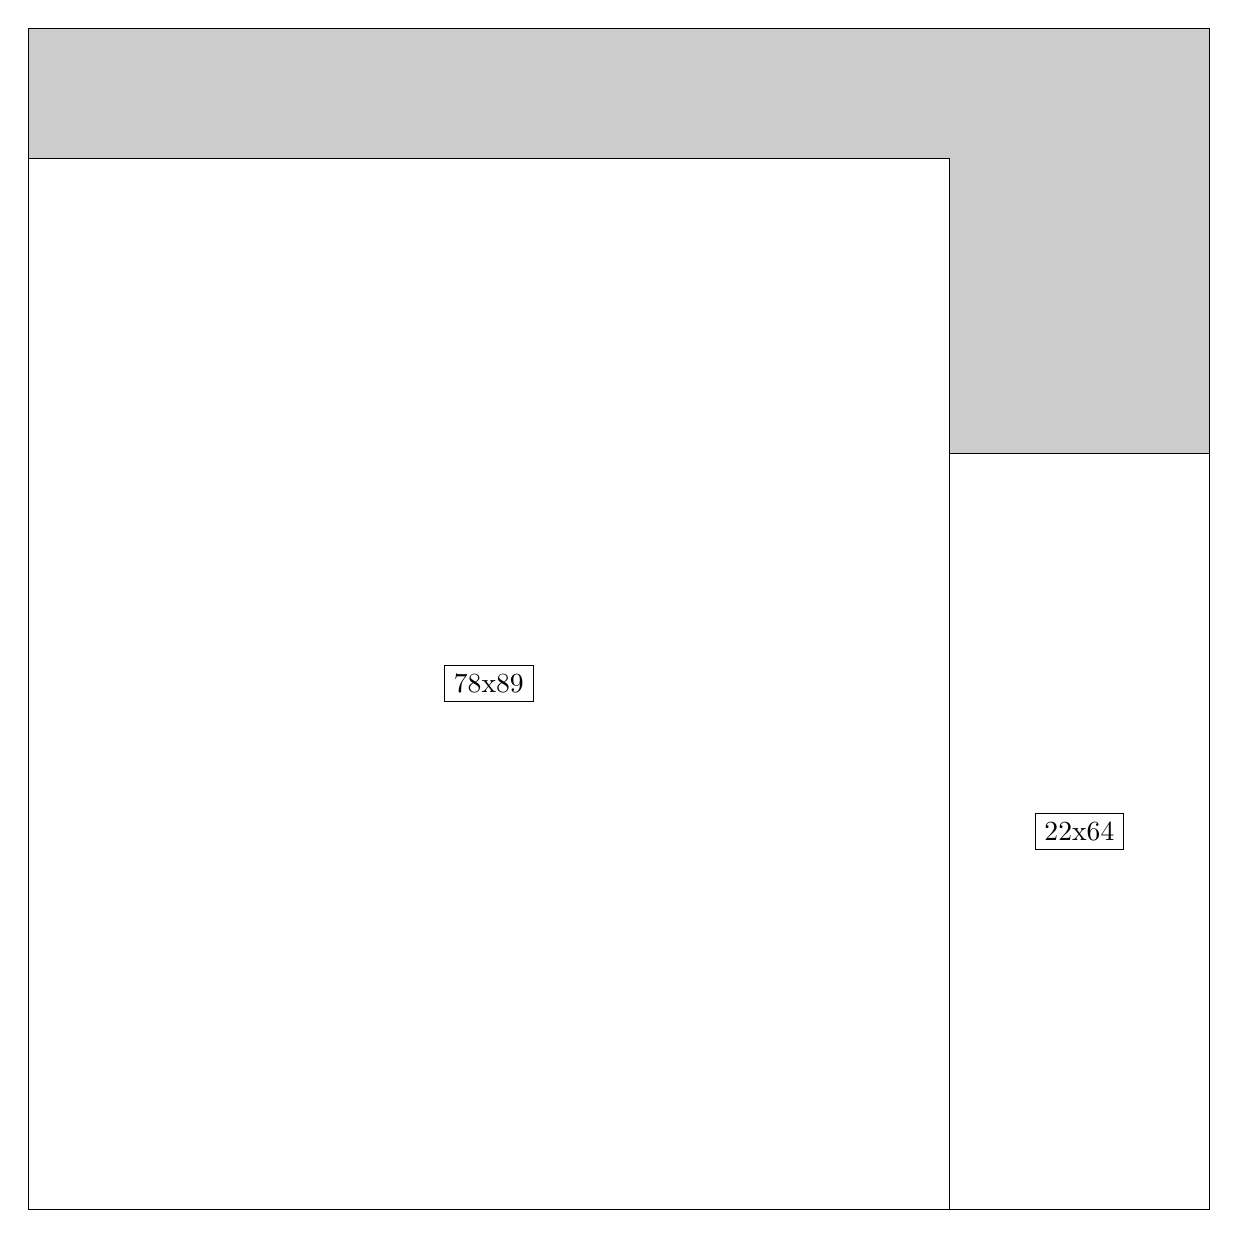
\begin{tikzpicture}[shorten >=1pt,scale=1.0,every node/.style={scale=1.0},->]
\tikzstyle{vertex}=[circle,fill=black!25,minimum size=14pt,inner sep=0pt]
\filldraw[fill=gray!40!white, draw=black] (0,0) rectangle (15.0,15.0);
\foreach \name/\x/\y/\w/\h in {78x89/0.0/0.0/11.7/13.35,22x64/11.7/0.0/3.3/9.6}
\filldraw[fill=white!40!white, draw=black] (\x,\y) rectangle node[draw] (\name) {\name} ++(\w,\h);
\end{tikzpicture}


w =78 , h =89 , x =0 , y =0 , v =6942
\par
w =22 , h =64 , x =78 , y =0 , v =1408
\par
\newpage


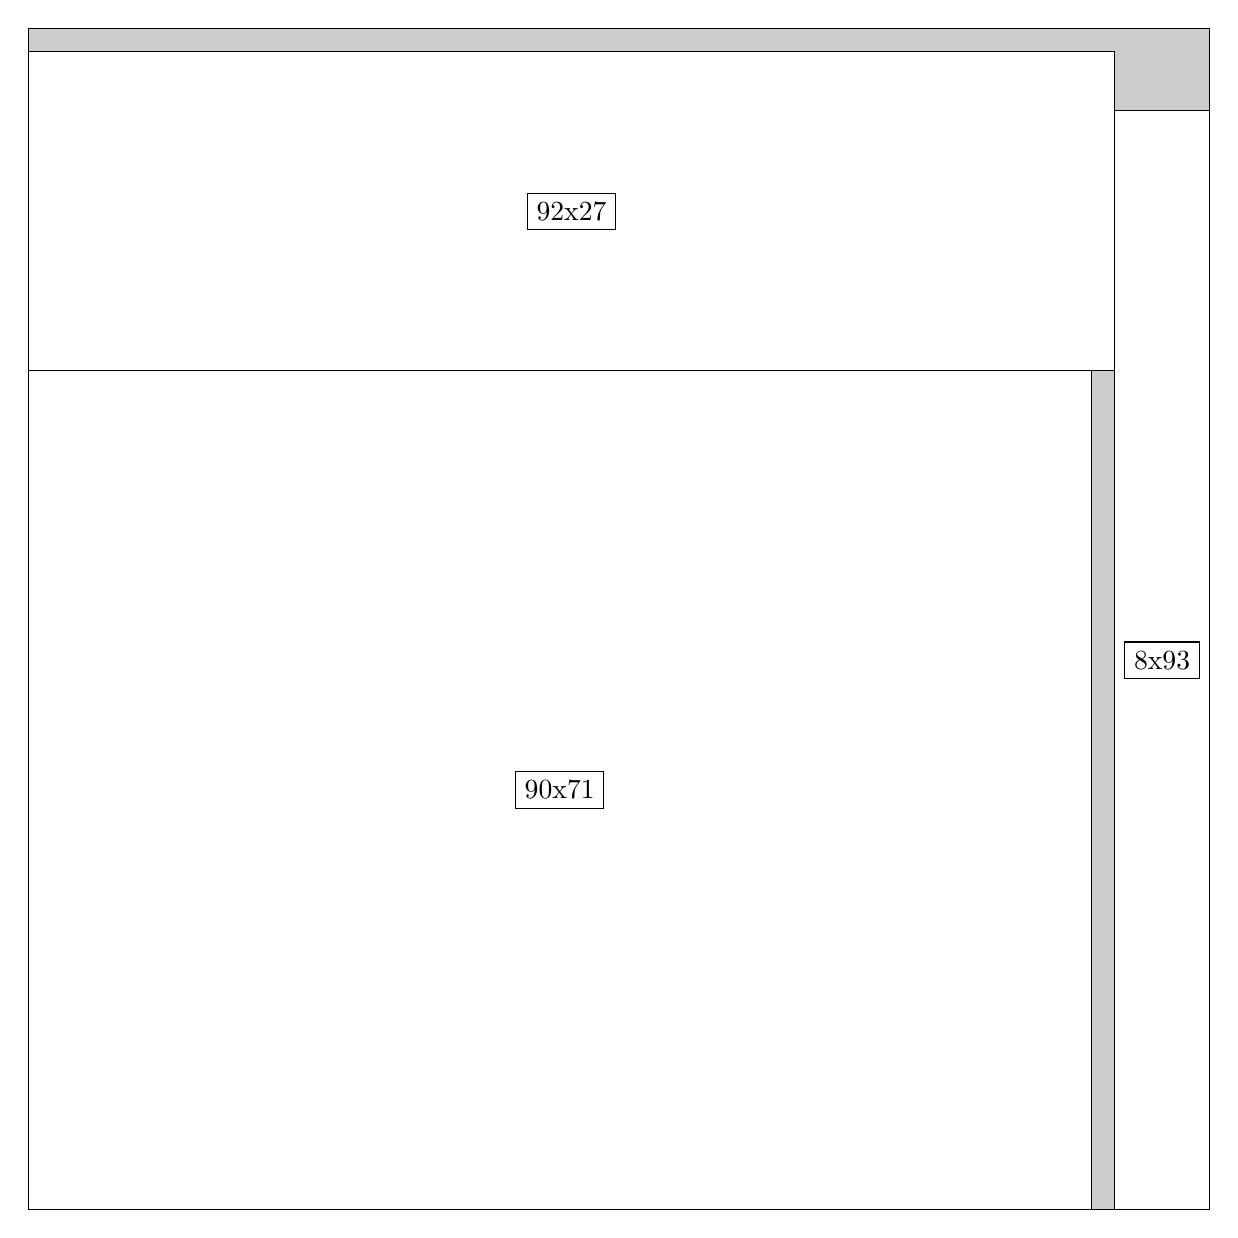
\begin{tikzpicture}[shorten >=1pt,scale=1.0,every node/.style={scale=1.0},->]
\tikzstyle{vertex}=[circle,fill=black!25,minimum size=14pt,inner sep=0pt]
\filldraw[fill=gray!40!white, draw=black] (0,0) rectangle (15.0,15.0);
\foreach \name/\x/\y/\w/\h in {90x71/0.0/0.0/13.5/10.65,92x27/0.0/10.65/13.799999999999999/4.05,8x93/13.799999999999999/0.0/1.2/13.95}
\filldraw[fill=white!40!white, draw=black] (\x,\y) rectangle node[draw] (\name) {\name} ++(\w,\h);
\end{tikzpicture}


w =90 , h =71 , x =0 , y =0 , v =6390
\par
w =92 , h =27 , x =0 , y =71 , v =2484
\par
w =8 , h =93 , x =92 , y =0 , v =744
\par
\newpage


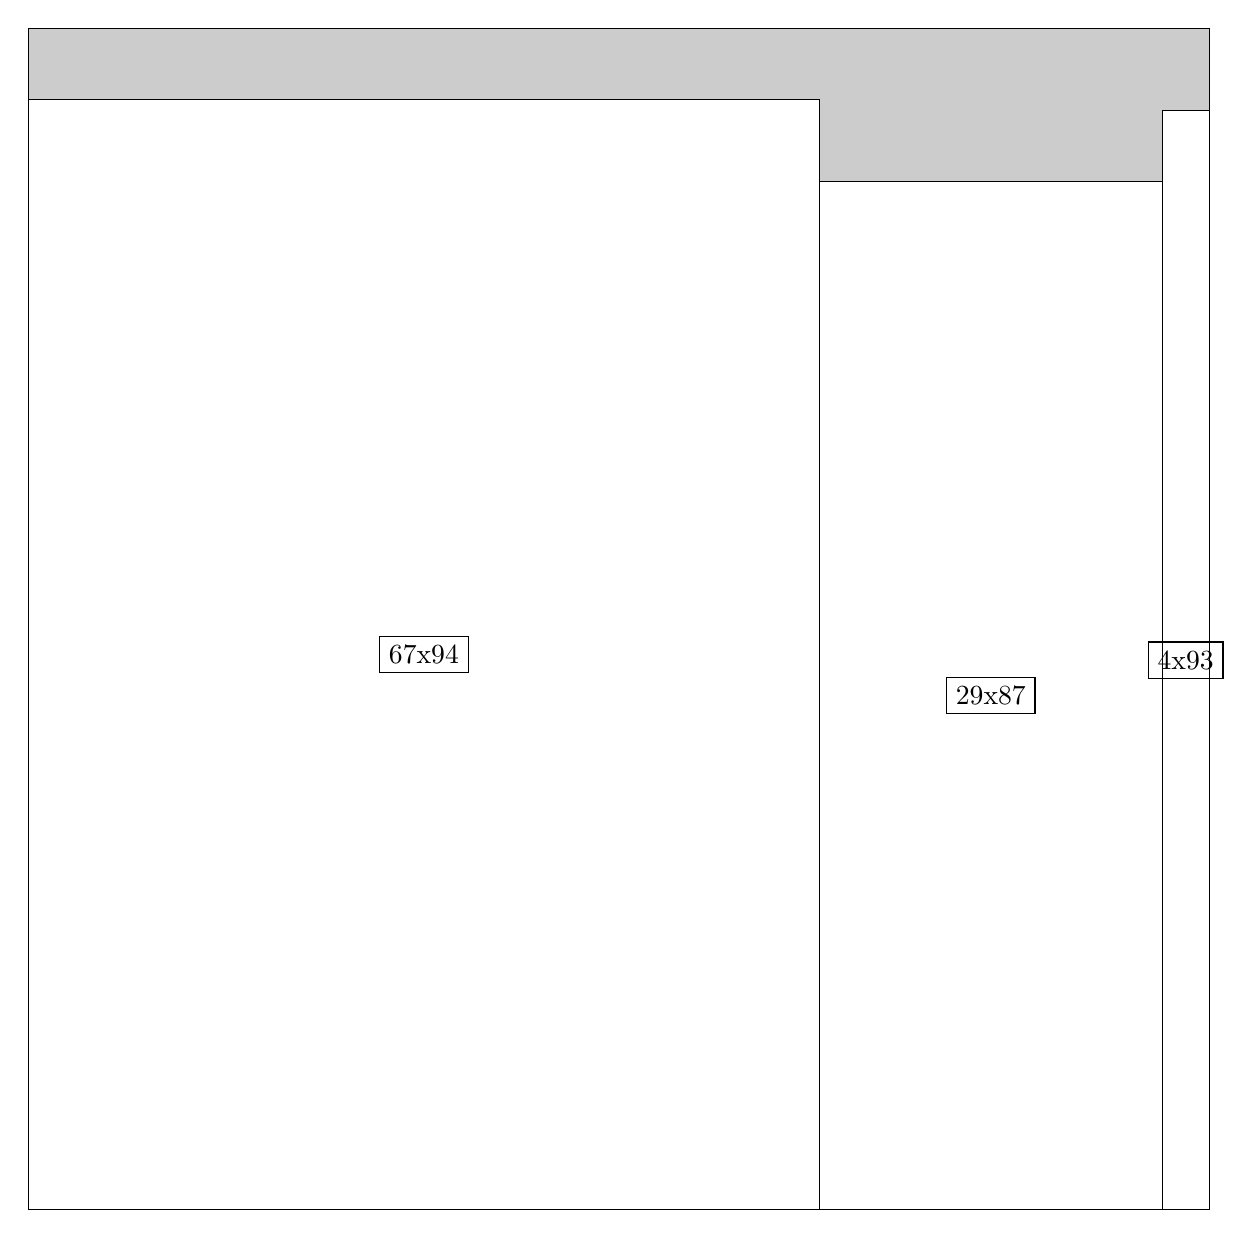
\begin{tikzpicture}[shorten >=1pt,scale=1.0,every node/.style={scale=1.0},->]
\tikzstyle{vertex}=[circle,fill=black!25,minimum size=14pt,inner sep=0pt]
\filldraw[fill=gray!40!white, draw=black] (0,0) rectangle (15.0,15.0);
\foreach \name/\x/\y/\w/\h in {67x94/0.0/0.0/10.049999999999999/14.1,29x87/10.049999999999999/0.0/4.35/13.049999999999999,4x93/14.399999999999999/0.0/0.6/13.95}
\filldraw[fill=white!40!white, draw=black] (\x,\y) rectangle node[draw] (\name) {\name} ++(\w,\h);
\end{tikzpicture}


w =67 , h =94 , x =0 , y =0 , v =6298
\par
w =29 , h =87 , x =67 , y =0 , v =2523
\par
w =4 , h =93 , x =96 , y =0 , v =372
\par
\newpage


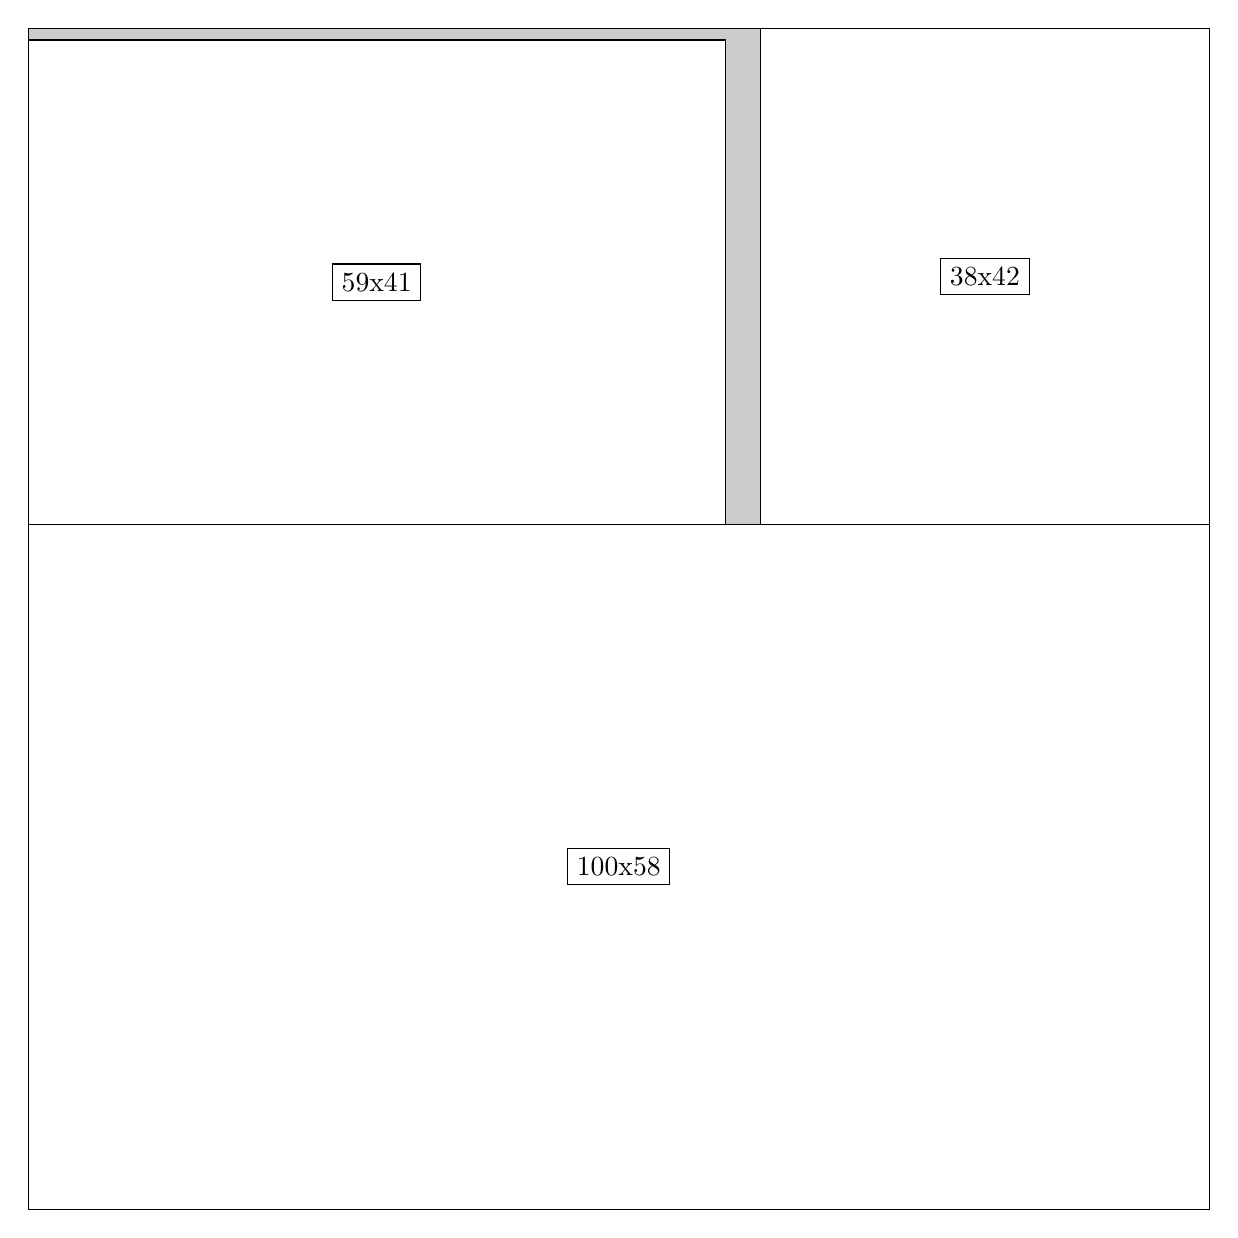
\begin{tikzpicture}[shorten >=1pt,scale=1.0,every node/.style={scale=1.0},->]
\tikzstyle{vertex}=[circle,fill=black!25,minimum size=14pt,inner sep=0pt]
\filldraw[fill=gray!40!white, draw=black] (0,0) rectangle (15.0,15.0);
\foreach \name/\x/\y/\w/\h in {100x58/0.0/0.0/15.0/8.7,59x41/0.0/8.7/8.85/6.1499999999999995,38x42/9.299999999999999/8.7/5.7/6.3}
\filldraw[fill=white!40!white, draw=black] (\x,\y) rectangle node[draw] (\name) {\name} ++(\w,\h);
\end{tikzpicture}


w =100 , h =58 , x =0 , y =0 , v =5800
\par
w =59 , h =41 , x =0 , y =58 , v =2419
\par
w =38 , h =42 , x =62 , y =58 , v =1596
\par
\newpage


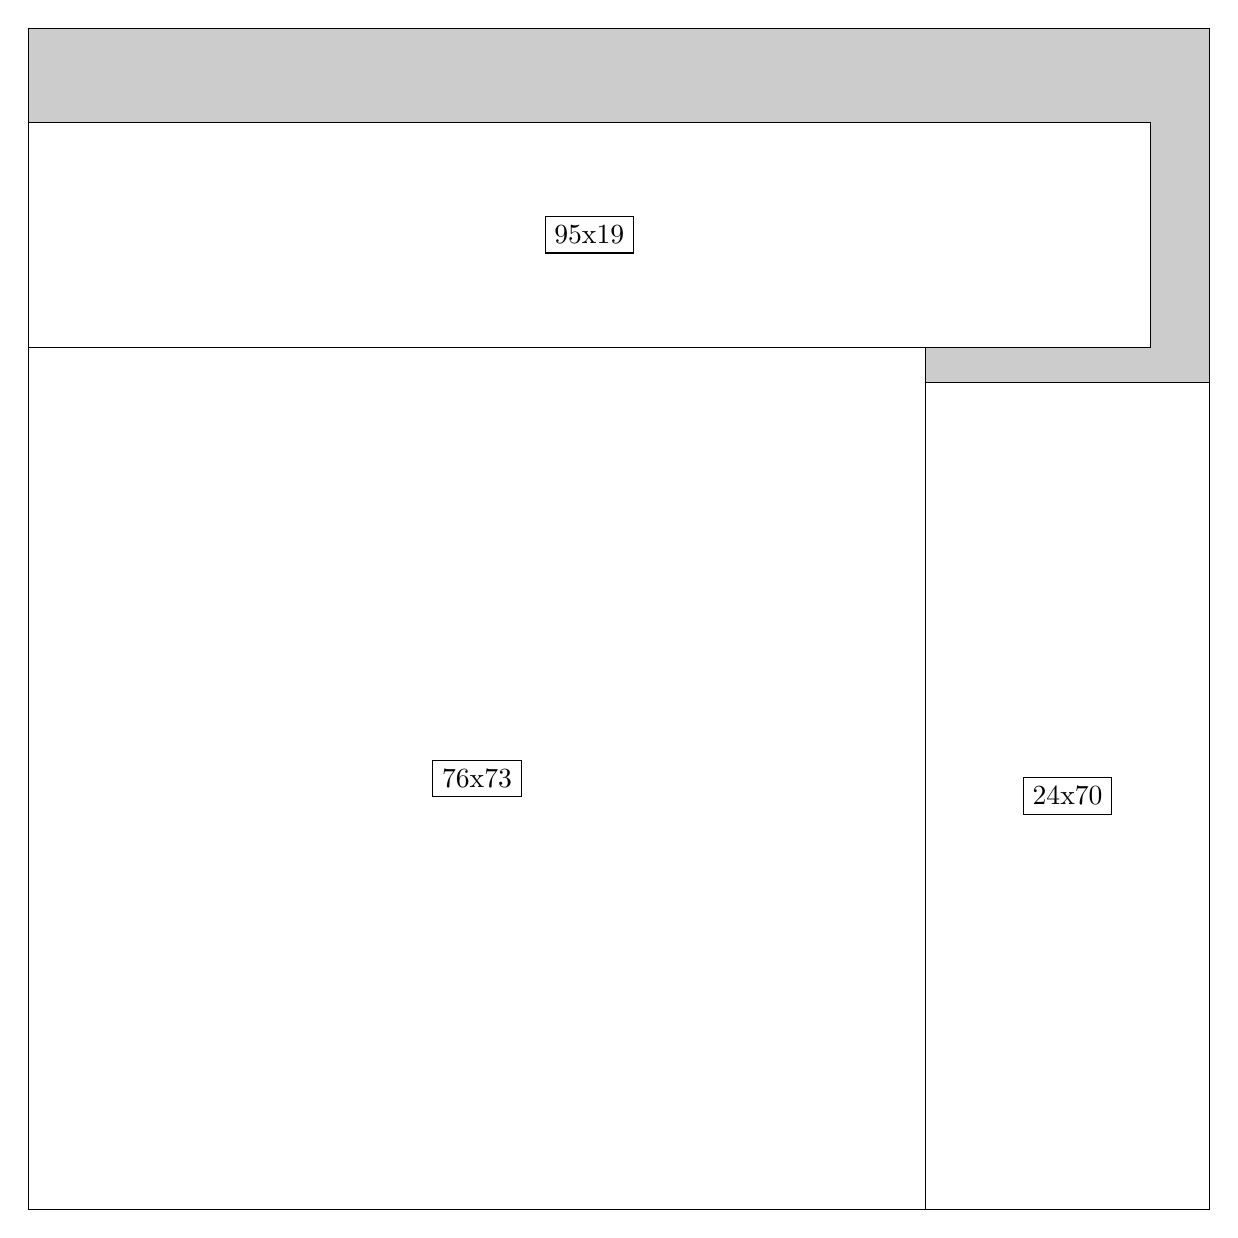
\begin{tikzpicture}[shorten >=1pt,scale=1.0,every node/.style={scale=1.0},->]
\tikzstyle{vertex}=[circle,fill=black!25,minimum size=14pt,inner sep=0pt]
\filldraw[fill=gray!40!white, draw=black] (0,0) rectangle (15.0,15.0);
\foreach \name/\x/\y/\w/\h in {76x73/0.0/0.0/11.4/10.95,95x19/0.0/10.95/14.25/2.85,24x70/11.4/0.0/3.5999999999999996/10.5}
\filldraw[fill=white!40!white, draw=black] (\x,\y) rectangle node[draw] (\name) {\name} ++(\w,\h);
\end{tikzpicture}


w =76 , h =73 , x =0 , y =0 , v =5548
\par
w =95 , h =19 , x =0 , y =73 , v =1805
\par
w =24 , h =70 , x =76 , y =0 , v =1680
\par
\newpage


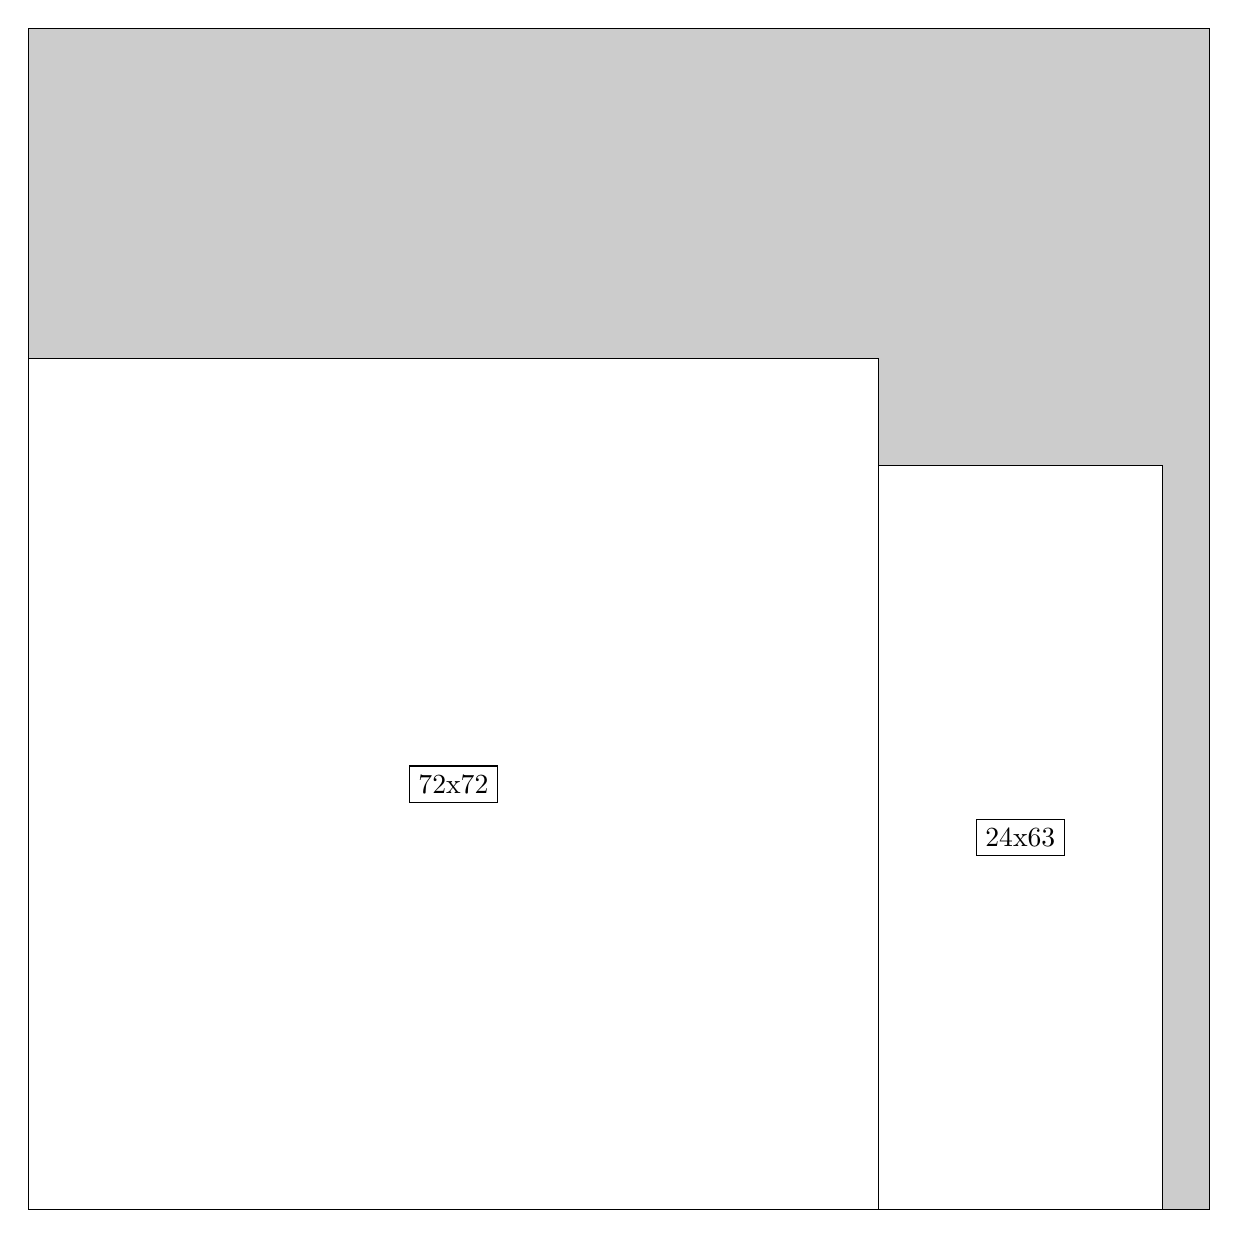
\begin{tikzpicture}[shorten >=1pt,scale=1.0,every node/.style={scale=1.0},->]
\tikzstyle{vertex}=[circle,fill=black!25,minimum size=14pt,inner sep=0pt]
\filldraw[fill=gray!40!white, draw=black] (0,0) rectangle (15.0,15.0);
\foreach \name/\x/\y/\w/\h in {72x72/0.0/0.0/10.799999999999999/10.799999999999999,24x63/10.799999999999999/0.0/3.5999999999999996/9.45}
\filldraw[fill=white!40!white, draw=black] (\x,\y) rectangle node[draw] (\name) {\name} ++(\w,\h);
\end{tikzpicture}


w =72 , h =72 , x =0 , y =0 , v =5184
\par
w =24 , h =63 , x =72 , y =0 , v =1512
\par
\newpage


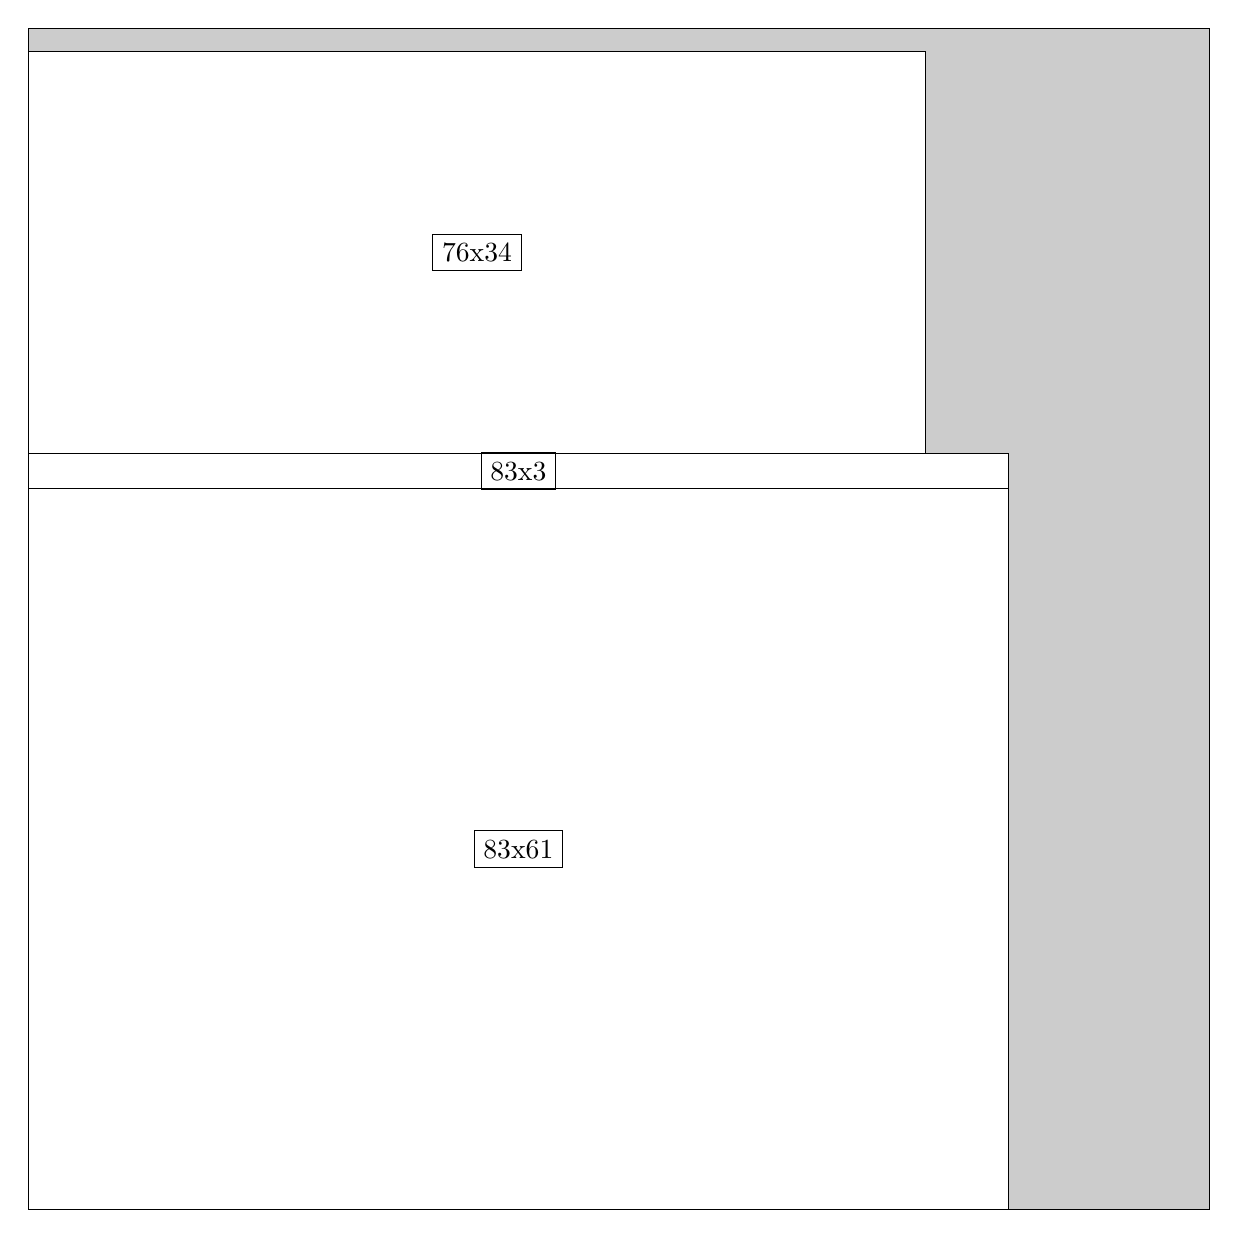
\begin{tikzpicture}[shorten >=1pt,scale=1.0,every node/.style={scale=1.0},->]
\tikzstyle{vertex}=[circle,fill=black!25,minimum size=14pt,inner sep=0pt]
\filldraw[fill=gray!40!white, draw=black] (0,0) rectangle (15.0,15.0);
\foreach \name/\x/\y/\w/\h in {83x61/0.0/0.0/12.45/9.15,76x34/0.0/9.6/11.4/5.1,83x3/0.0/9.15/12.45/0.44999999999999996}
\filldraw[fill=white!40!white, draw=black] (\x,\y) rectangle node[draw] (\name) {\name} ++(\w,\h);
\end{tikzpicture}


w =83 , h =61 , x =0 , y =0 , v =5063
\par
w =76 , h =34 , x =0 , y =64 , v =2584
\par
w =83 , h =3 , x =0 , y =61 , v =249
\par
\newpage


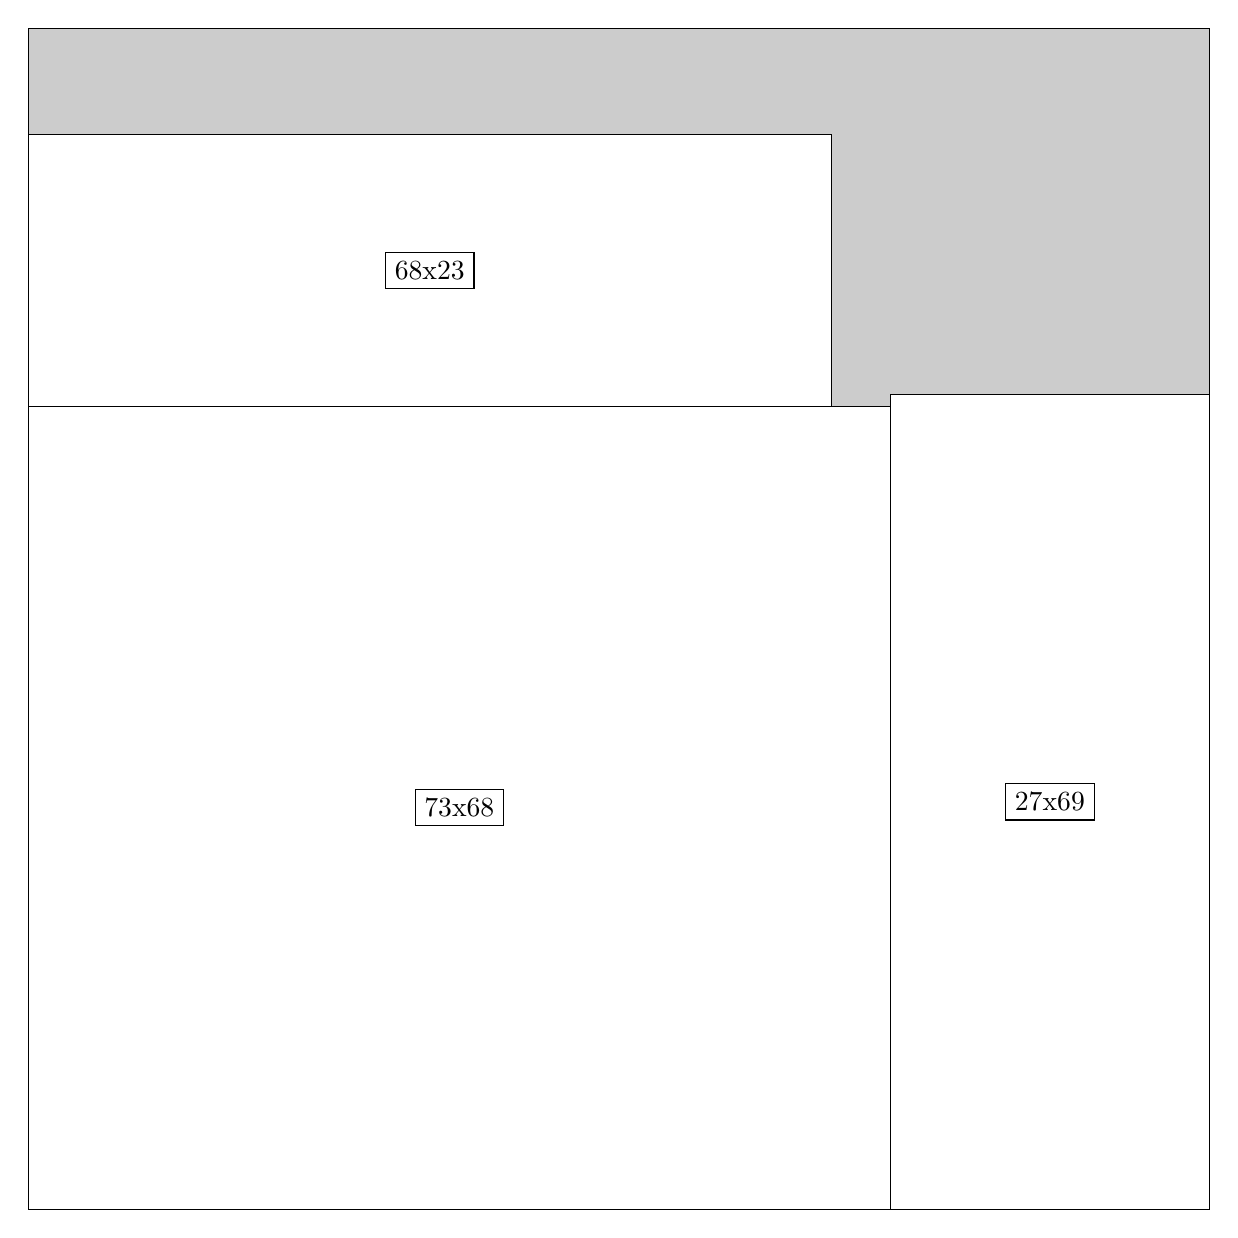
\begin{tikzpicture}[shorten >=1pt,scale=1.0,every node/.style={scale=1.0},->]
\tikzstyle{vertex}=[circle,fill=black!25,minimum size=14pt,inner sep=0pt]
\filldraw[fill=gray!40!white, draw=black] (0,0) rectangle (15.0,15.0);
\foreach \name/\x/\y/\w/\h in {73x68/0.0/0.0/10.95/10.2,27x69/10.95/0.0/4.05/10.35,68x23/0.0/10.2/10.2/3.4499999999999997}
\filldraw[fill=white!40!white, draw=black] (\x,\y) rectangle node[draw] (\name) {\name} ++(\w,\h);
\end{tikzpicture}


w =73 , h =68 , x =0 , y =0 , v =4964
\par
w =27 , h =69 , x =73 , y =0 , v =1863
\par
w =68 , h =23 , x =0 , y =68 , v =1564
\par
\newpage


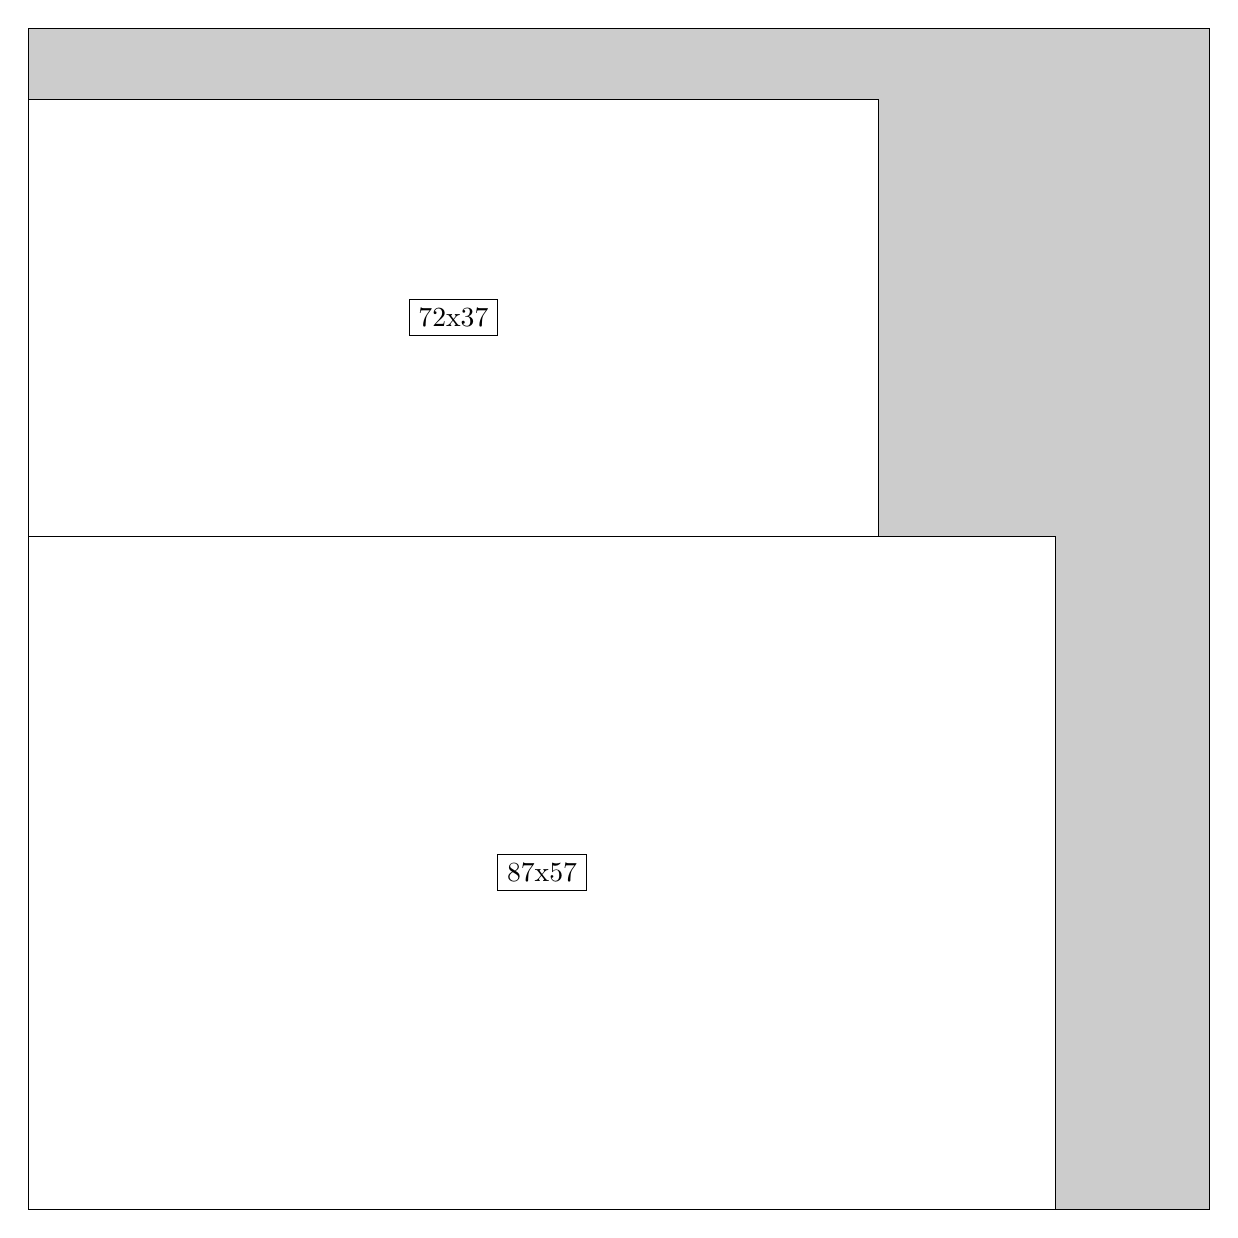
\begin{tikzpicture}[shorten >=1pt,scale=1.0,every node/.style={scale=1.0},->]
\tikzstyle{vertex}=[circle,fill=black!25,minimum size=14pt,inner sep=0pt]
\filldraw[fill=gray!40!white, draw=black] (0,0) rectangle (15.0,15.0);
\foreach \name/\x/\y/\w/\h in {87x57/0.0/0.0/13.049999999999999/8.549999999999999,72x37/0.0/8.549999999999999/10.799999999999999/5.55}
\filldraw[fill=white!40!white, draw=black] (\x,\y) rectangle node[draw] (\name) {\name} ++(\w,\h);
\end{tikzpicture}


w =87 , h =57 , x =0 , y =0 , v =4959
\par
w =72 , h =37 , x =0 , y =57 , v =2664
\par
\newpage


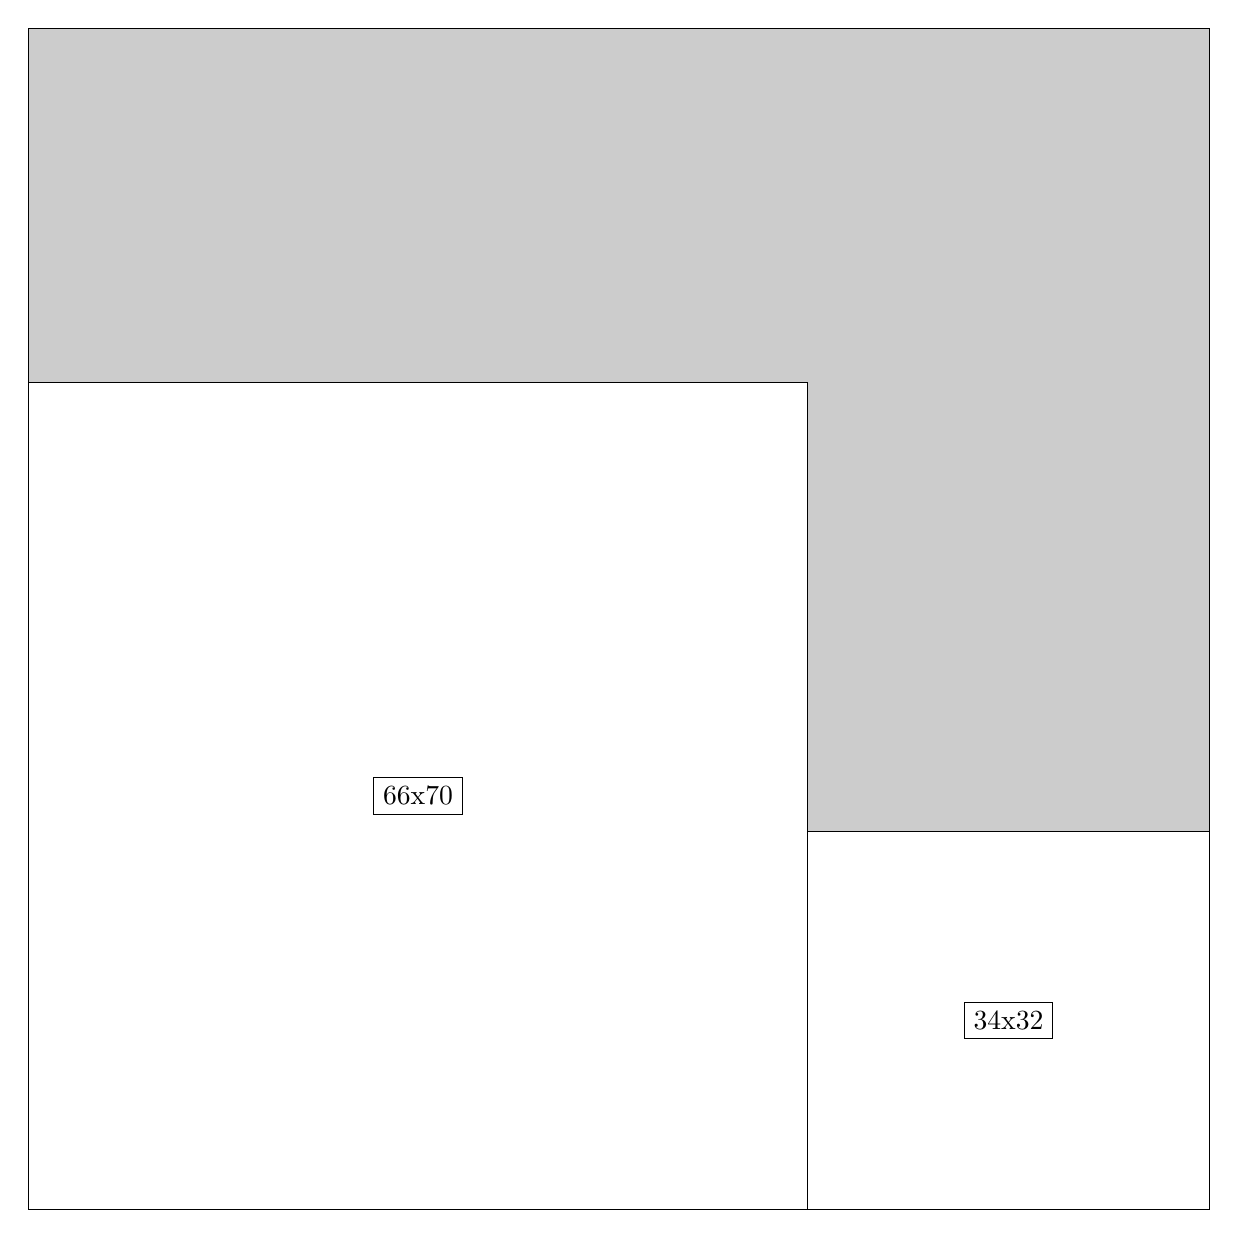
\begin{tikzpicture}[shorten >=1pt,scale=1.0,every node/.style={scale=1.0},->]
\tikzstyle{vertex}=[circle,fill=black!25,minimum size=14pt,inner sep=0pt]
\filldraw[fill=gray!40!white, draw=black] (0,0) rectangle (15.0,15.0);
\foreach \name/\x/\y/\w/\h in {66x70/0.0/0.0/9.9/10.5,34x32/9.9/0.0/5.1/4.8}
\filldraw[fill=white!40!white, draw=black] (\x,\y) rectangle node[draw] (\name) {\name} ++(\w,\h);
\end{tikzpicture}


w =66 , h =70 , x =0 , y =0 , v =4620
\par
w =34 , h =32 , x =66 , y =0 , v =1088
\par
\newpage


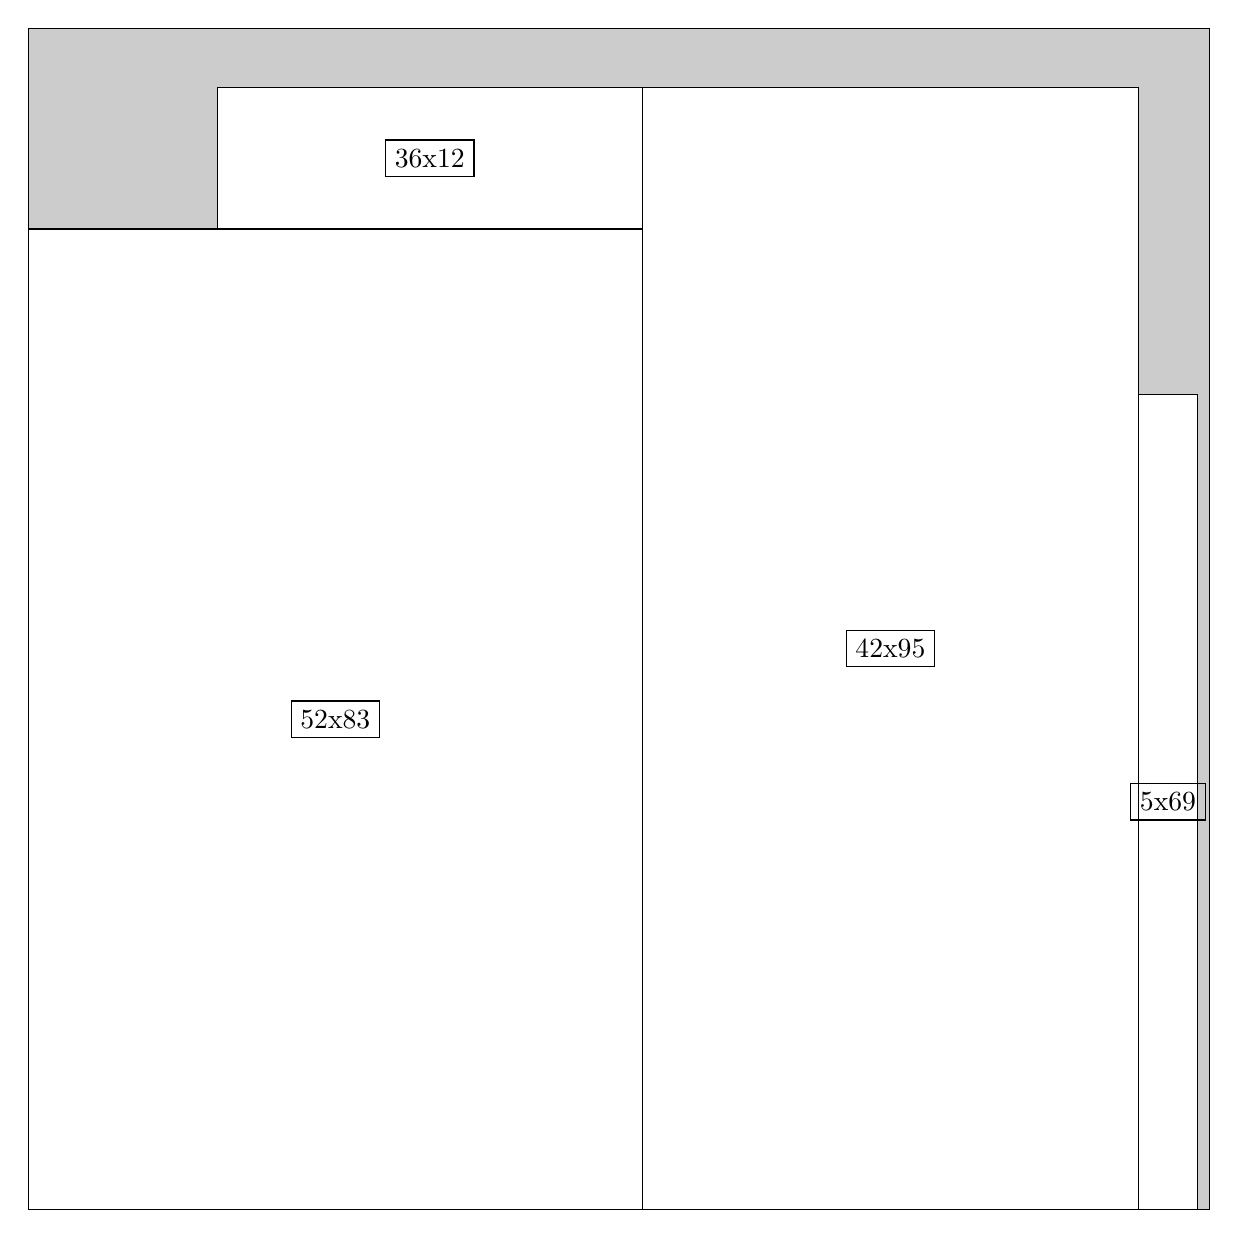
\begin{tikzpicture}[shorten >=1pt,scale=1.0,every node/.style={scale=1.0},->]
\tikzstyle{vertex}=[circle,fill=black!25,minimum size=14pt,inner sep=0pt]
\filldraw[fill=gray!40!white, draw=black] (0,0) rectangle (15.0,15.0);
\foreach \name/\x/\y/\w/\h in {52x83/0.0/0.0/7.8/12.45,42x95/7.8/0.0/6.3/14.25,36x12/2.4/12.45/5.3999999999999995/1.7999999999999998,5x69/14.1/0.0/0.75/10.35}
\filldraw[fill=white!40!white, draw=black] (\x,\y) rectangle node[draw] (\name) {\name} ++(\w,\h);
\end{tikzpicture}


w =52 , h =83 , x =0 , y =0 , v =4316
\par
w =42 , h =95 , x =52 , y =0 , v =3990
\par
w =36 , h =12 , x =16 , y =83 , v =432
\par
w =5 , h =69 , x =94 , y =0 , v =345
\par
\newpage


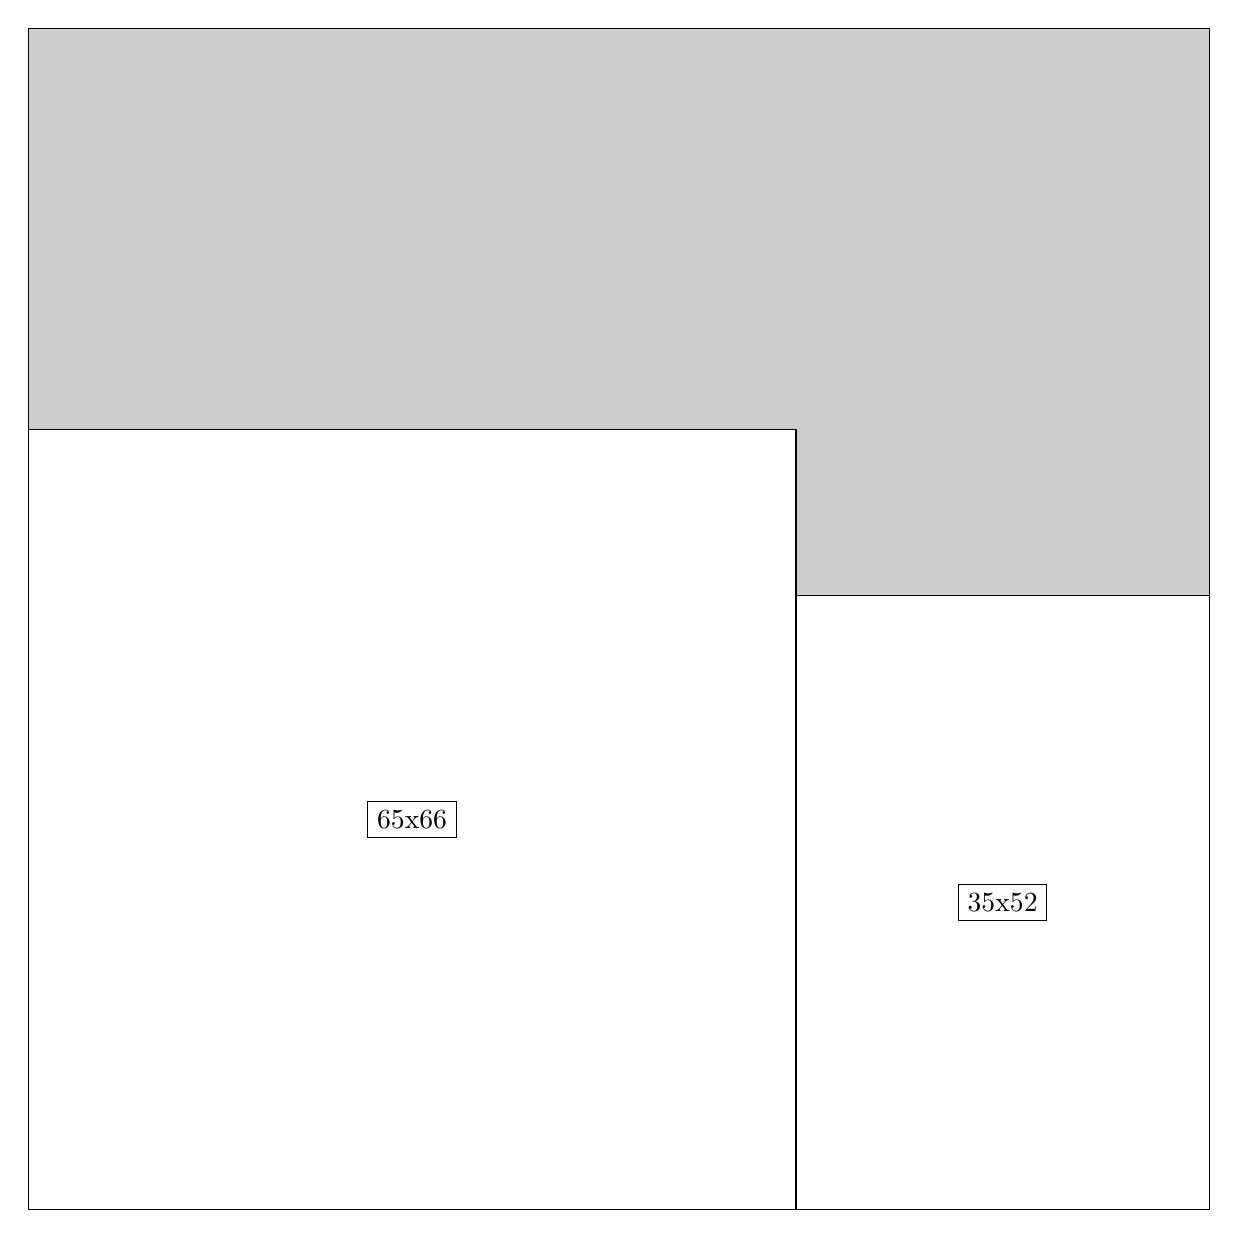
\begin{tikzpicture}[shorten >=1pt,scale=1.0,every node/.style={scale=1.0},->]
\tikzstyle{vertex}=[circle,fill=black!25,minimum size=14pt,inner sep=0pt]
\filldraw[fill=gray!40!white, draw=black] (0,0) rectangle (15.0,15.0);
\foreach \name/\x/\y/\w/\h in {65x66/0.0/0.0/9.75/9.9,35x52/9.75/0.0/5.25/7.8}
\filldraw[fill=white!40!white, draw=black] (\x,\y) rectangle node[draw] (\name) {\name} ++(\w,\h);
\end{tikzpicture}


w =65 , h =66 , x =0 , y =0 , v =4290
\par
w =35 , h =52 , x =65 , y =0 , v =1820
\par
\newpage


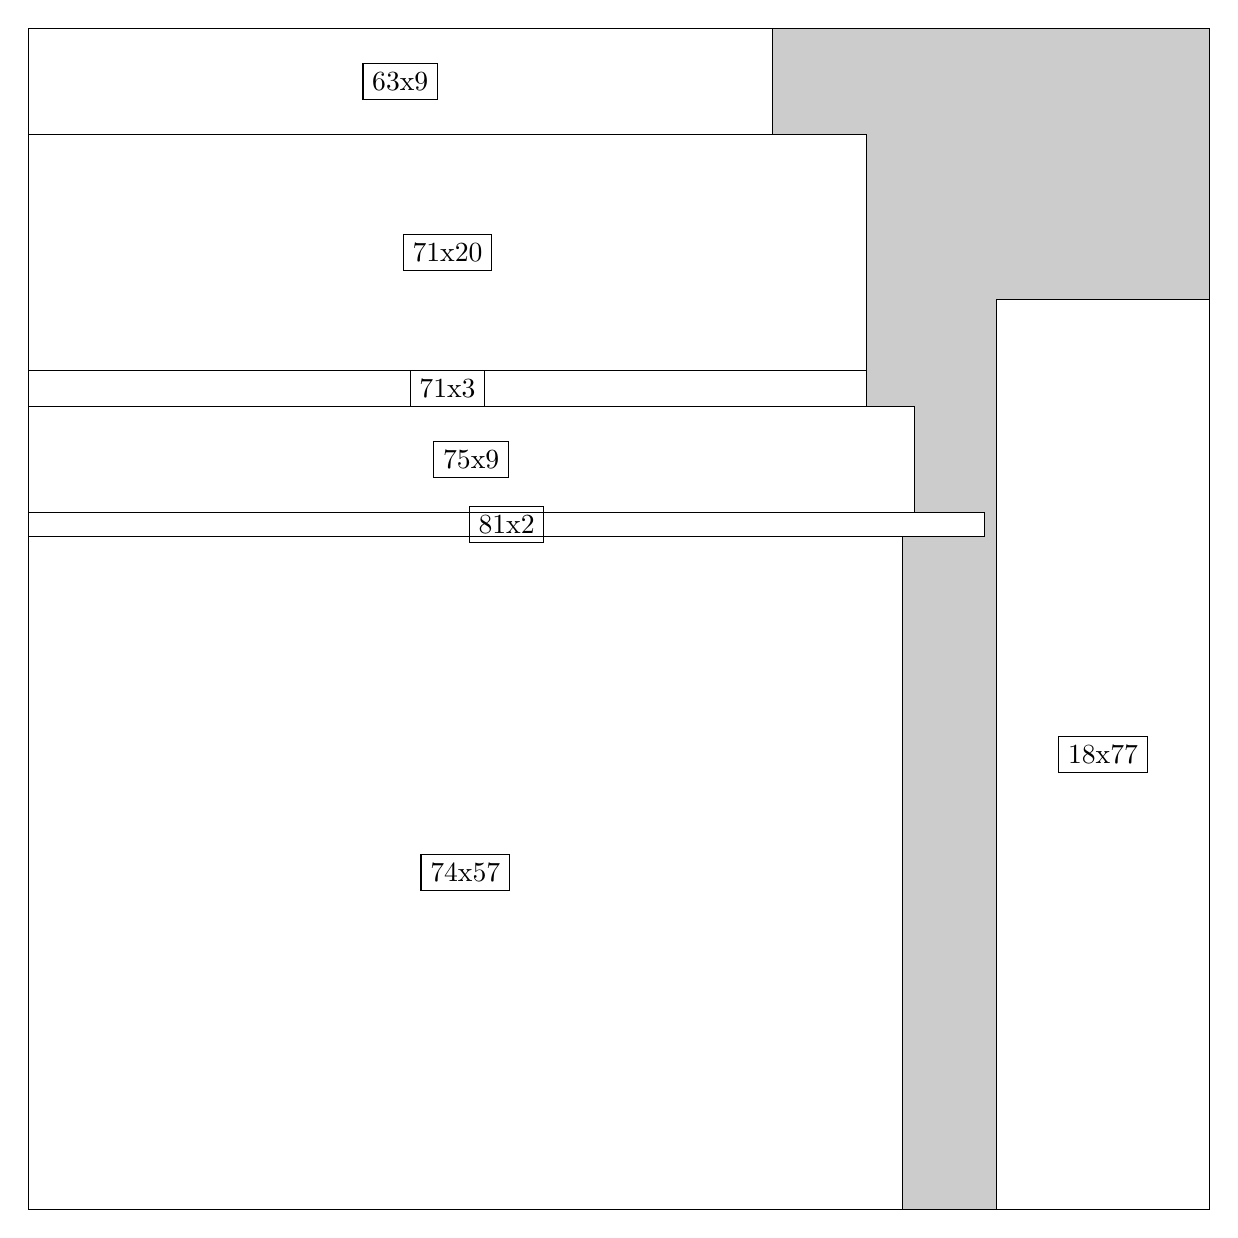
\begin{tikzpicture}[shorten >=1pt,scale=1.0,every node/.style={scale=1.0},->]
\tikzstyle{vertex}=[circle,fill=black!25,minimum size=14pt,inner sep=0pt]
\filldraw[fill=gray!40!white, draw=black] (0,0) rectangle (15.0,15.0);
\foreach \name/\x/\y/\w/\h in {74x57/0.0/0.0/11.1/8.549999999999999,71x20/0.0/10.65/10.65/3.0,18x77/12.299999999999999/0.0/2.6999999999999997/11.549999999999999,75x9/0.0/8.85/11.25/1.3499999999999999,63x9/0.0/13.65/9.45/1.3499999999999999,71x3/0.0/10.2/10.65/0.44999999999999996,81x2/0.0/8.549999999999999/12.15/0.3}
\filldraw[fill=white!40!white, draw=black] (\x,\y) rectangle node[draw] (\name) {\name} ++(\w,\h);
\end{tikzpicture}


w =74 , h =57 , x =0 , y =0 , v =4218
\par
w =71 , h =20 , x =0 , y =71 , v =1420
\par
w =18 , h =77 , x =82 , y =0 , v =1386
\par
w =75 , h =9 , x =0 , y =59 , v =675
\par
w =63 , h =9 , x =0 , y =91 , v =567
\par
w =71 , h =3 , x =0 , y =68 , v =213
\par
w =81 , h =2 , x =0 , y =57 , v =162
\par
\newpage


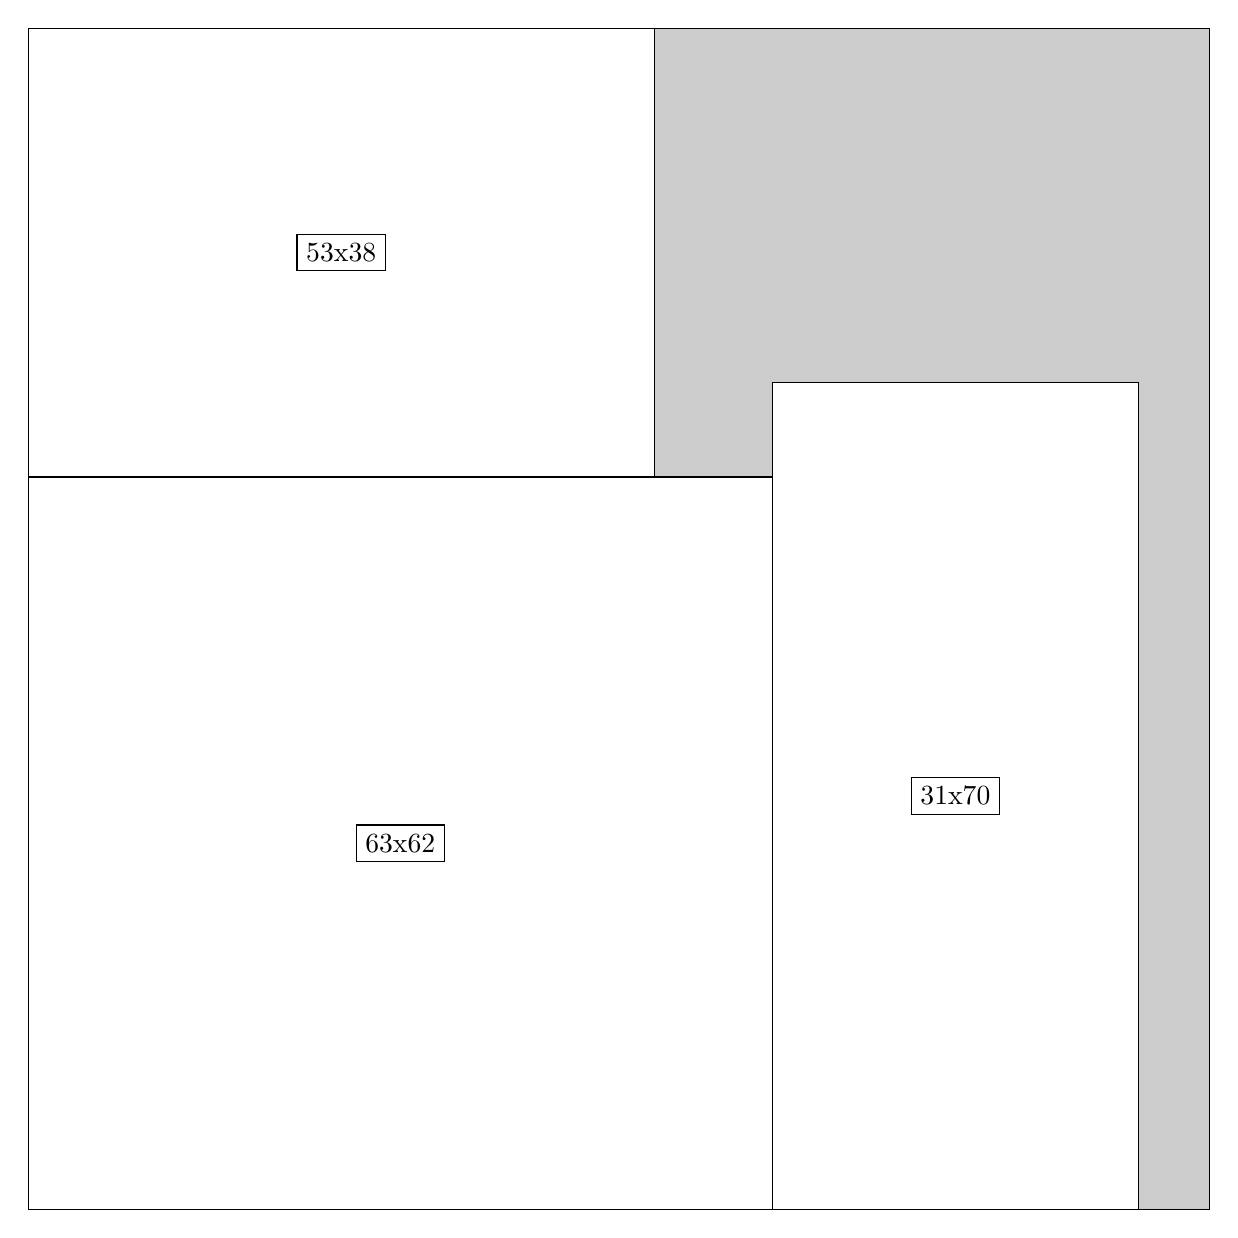
\begin{tikzpicture}[shorten >=1pt,scale=1.0,every node/.style={scale=1.0},->]
\tikzstyle{vertex}=[circle,fill=black!25,minimum size=14pt,inner sep=0pt]
\filldraw[fill=gray!40!white, draw=black] (0,0) rectangle (15.0,15.0);
\foreach \name/\x/\y/\w/\h in {63x62/0.0/0.0/9.45/9.299999999999999,31x70/9.45/0.0/4.6499999999999995/10.5,53x38/0.0/9.299999999999999/7.949999999999999/5.7}
\filldraw[fill=white!40!white, draw=black] (\x,\y) rectangle node[draw] (\name) {\name} ++(\w,\h);
\end{tikzpicture}


w =63 , h =62 , x =0 , y =0 , v =3906
\par
w =31 , h =70 , x =63 , y =0 , v =2170
\par
w =53 , h =38 , x =0 , y =62 , v =2014
\par
\newpage


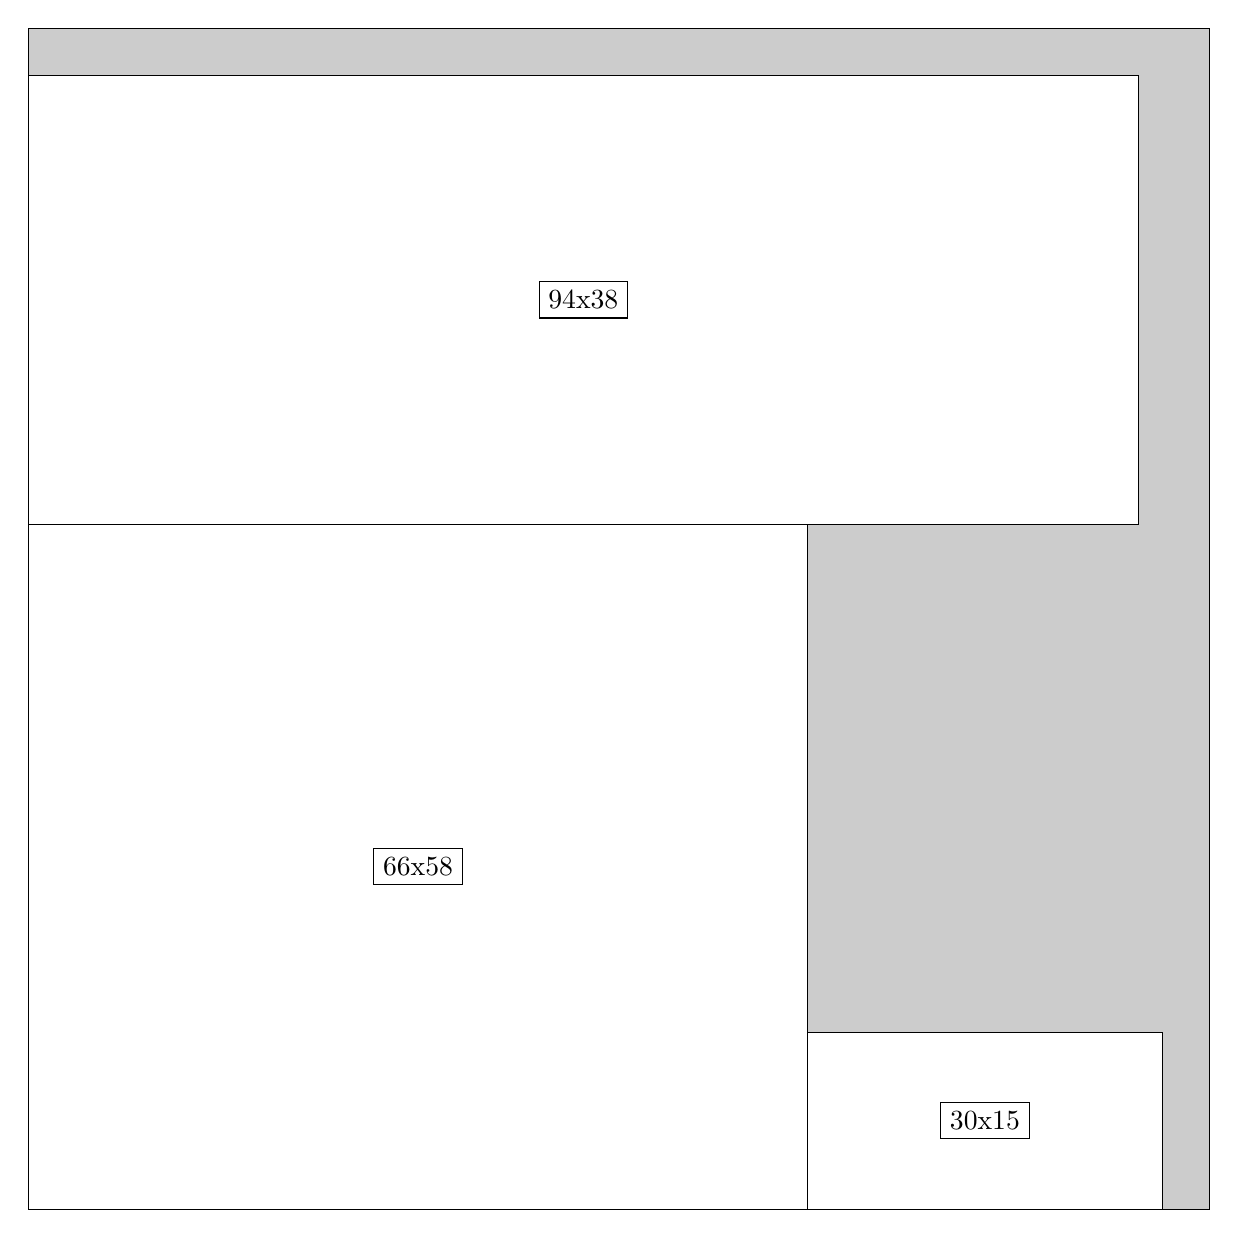
\begin{tikzpicture}[shorten >=1pt,scale=1.0,every node/.style={scale=1.0},->]
\tikzstyle{vertex}=[circle,fill=black!25,minimum size=14pt,inner sep=0pt]
\filldraw[fill=gray!40!white, draw=black] (0,0) rectangle (15.0,15.0);
\foreach \name/\x/\y/\w/\h in {66x58/0.0/0.0/9.9/8.7,30x15/9.9/0.0/4.5/2.25,94x38/0.0/8.7/14.1/5.7}
\filldraw[fill=white!40!white, draw=black] (\x,\y) rectangle node[draw] (\name) {\name} ++(\w,\h);
\end{tikzpicture}


w =66 , h =58 , x =0 , y =0 , v =3828
\par
w =30 , h =15 , x =66 , y =0 , v =450
\par
w =94 , h =38 , x =0 , y =58 , v =3572
\par
\newpage


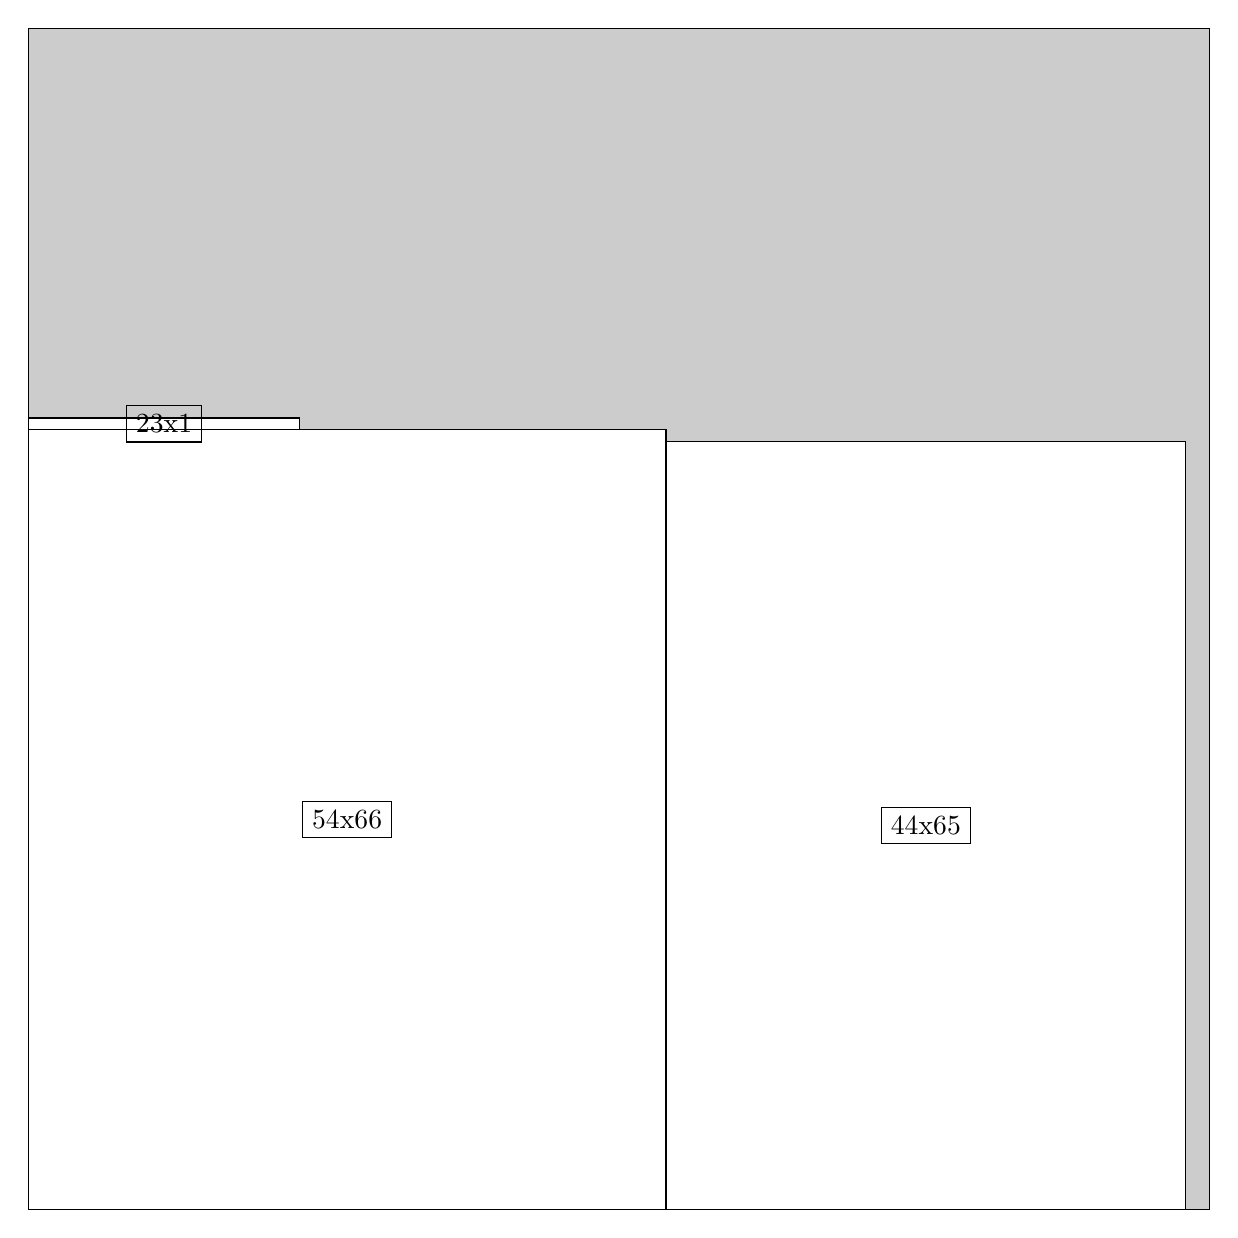
\begin{tikzpicture}[shorten >=1pt,scale=1.0,every node/.style={scale=1.0},->]
\tikzstyle{vertex}=[circle,fill=black!25,minimum size=14pt,inner sep=0pt]
\filldraw[fill=gray!40!white, draw=black] (0,0) rectangle (15.0,15.0);
\foreach \name/\x/\y/\w/\h in {54x66/0.0/0.0/8.1/9.9,44x65/8.1/0.0/6.6/9.75,23x1/0.0/9.9/3.4499999999999997/0.15}
\filldraw[fill=white!40!white, draw=black] (\x,\y) rectangle node[draw] (\name) {\name} ++(\w,\h);
\end{tikzpicture}


w =54 , h =66 , x =0 , y =0 , v =3564
\par
w =44 , h =65 , x =54 , y =0 , v =2860
\par
w =23 , h =1 , x =0 , y =66 , v =23
\par
\newpage


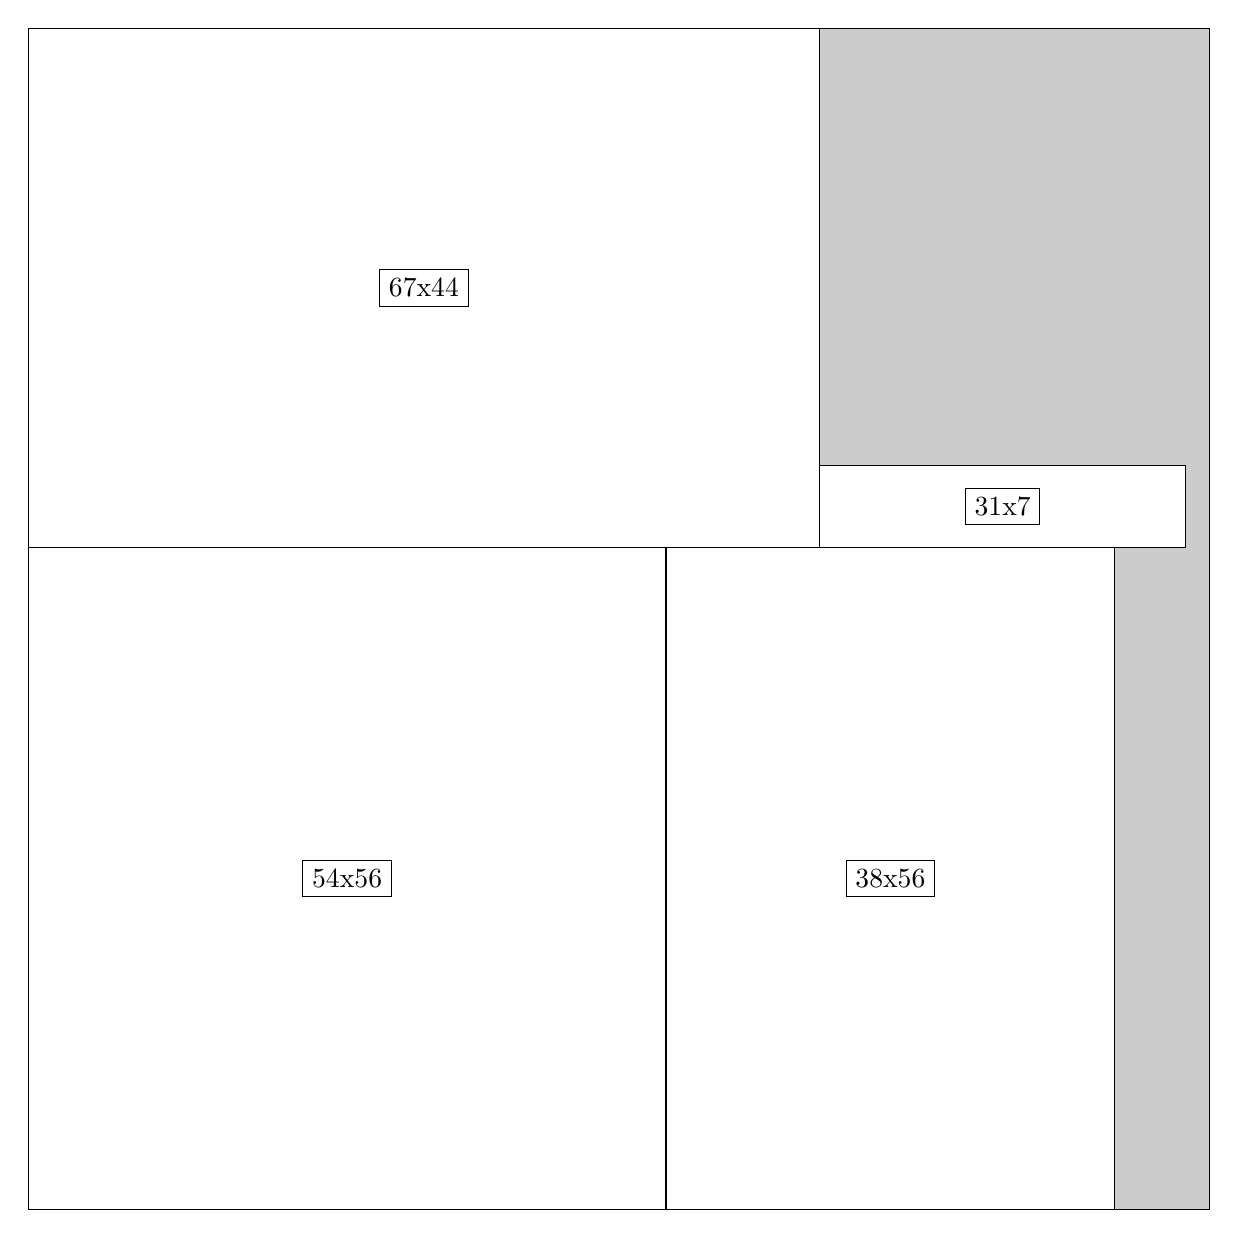
\begin{tikzpicture}[shorten >=1pt,scale=1.0,every node/.style={scale=1.0},->]
\tikzstyle{vertex}=[circle,fill=black!25,minimum size=14pt,inner sep=0pt]
\filldraw[fill=gray!40!white, draw=black] (0,0) rectangle (15.0,15.0);
\foreach \name/\x/\y/\w/\h in {54x56/0.0/0.0/8.1/8.4,67x44/0.0/8.4/10.049999999999999/6.6,38x56/8.1/0.0/5.7/8.4,31x7/10.049999999999999/8.4/4.6499999999999995/1.05}
\filldraw[fill=white!40!white, draw=black] (\x,\y) rectangle node[draw] (\name) {\name} ++(\w,\h);
\end{tikzpicture}


w =54 , h =56 , x =0 , y =0 , v =3024
\par
w =67 , h =44 , x =0 , y =56 , v =2948
\par
w =38 , h =56 , x =54 , y =0 , v =2128
\par
w =31 , h =7 , x =67 , y =56 , v =217
\par
\newpage


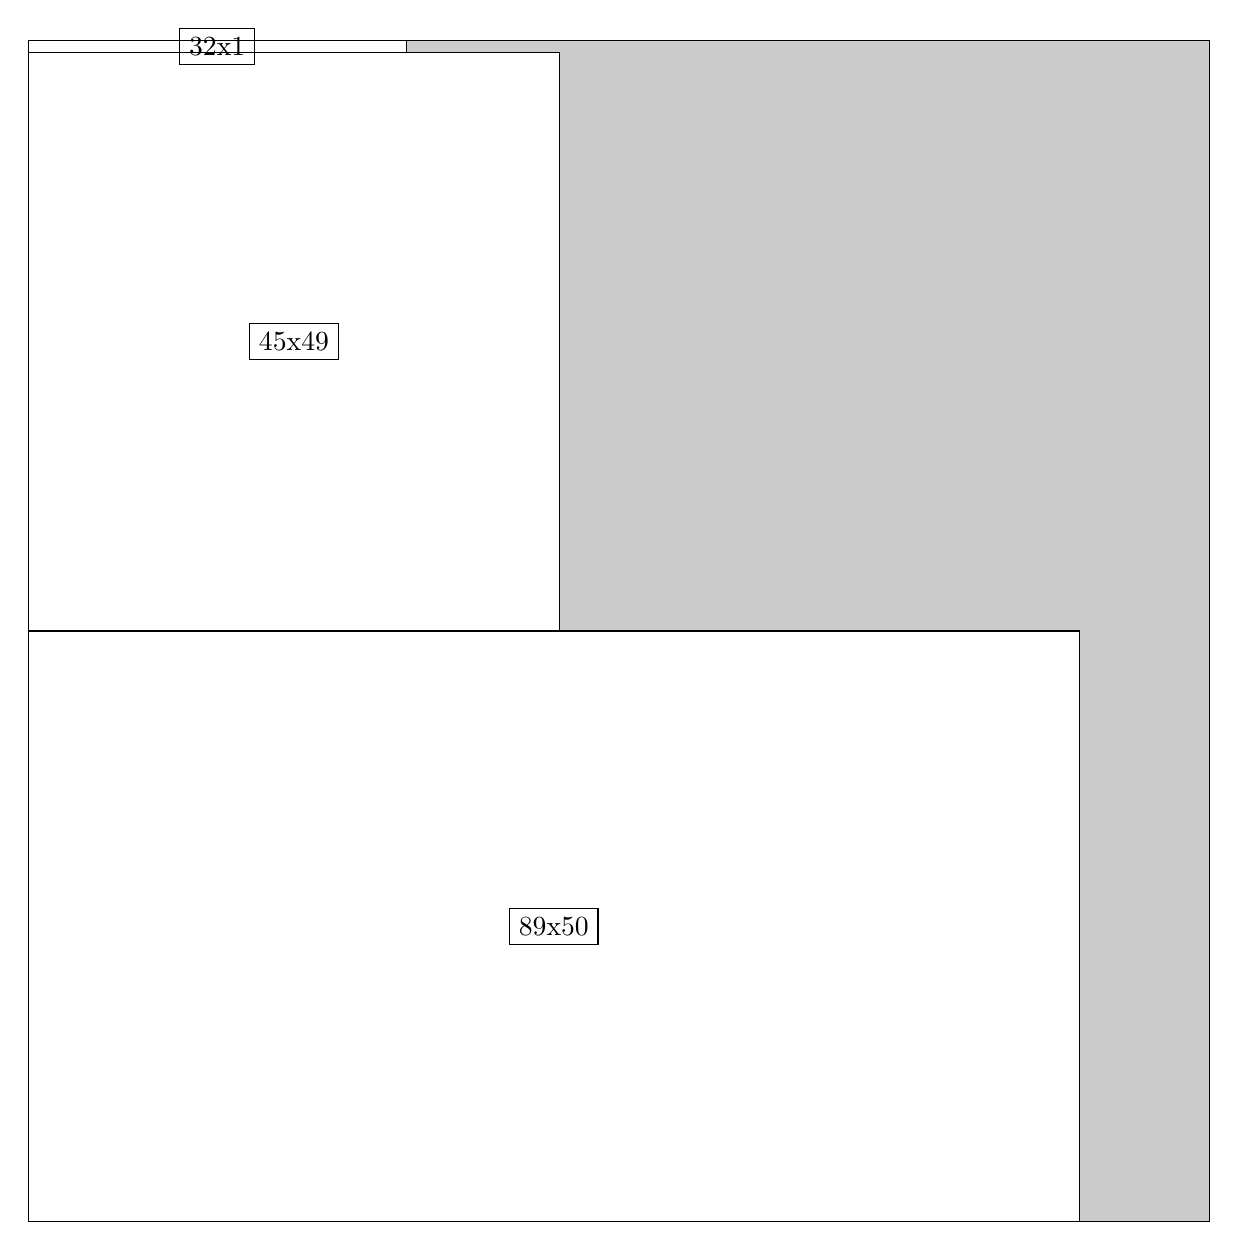
\begin{tikzpicture}[shorten >=1pt,scale=1.0,every node/.style={scale=1.0},->]
\tikzstyle{vertex}=[circle,fill=black!25,minimum size=14pt,inner sep=0pt]
\filldraw[fill=gray!40!white, draw=black] (0,0) rectangle (15.0,15.0);
\foreach \name/\x/\y/\w/\h in {89x50/0.0/0.0/13.35/7.5,45x49/0.0/7.5/6.75/7.35,32x1/0.0/14.85/4.8/0.15}
\filldraw[fill=white!40!white, draw=black] (\x,\y) rectangle node[draw] (\name) {\name} ++(\w,\h);
\end{tikzpicture}


w =89 , h =50 , x =0 , y =0 , v =4450
\par
w =45 , h =49 , x =0 , y =50 , v =2205
\par
w =32 , h =1 , x =0 , y =99 , v =32
\par
\newpage


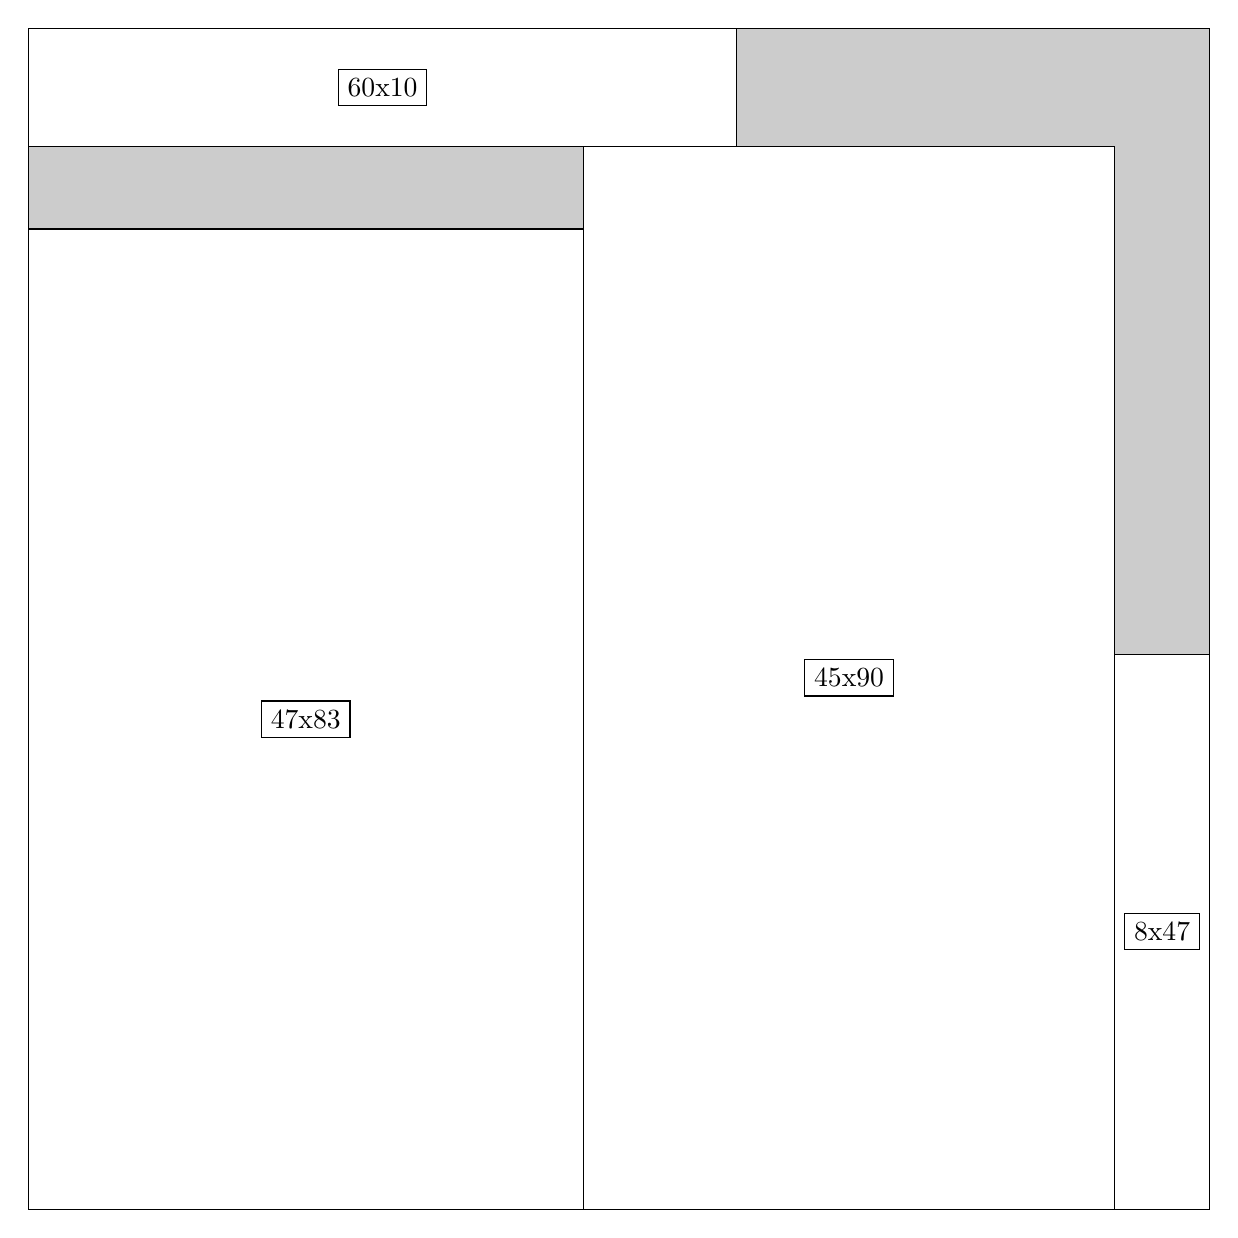
\begin{tikzpicture}[shorten >=1pt,scale=1.0,every node/.style={scale=1.0},->]
\tikzstyle{vertex}=[circle,fill=black!25,minimum size=14pt,inner sep=0pt]
\filldraw[fill=gray!40!white, draw=black] (0,0) rectangle (15.0,15.0);
\foreach \name/\x/\y/\w/\h in {47x83/0.0/0.0/7.05/12.45,45x90/7.05/0.0/6.75/13.5,60x10/0.0/13.5/9.0/1.5,8x47/13.799999999999999/0.0/1.2/7.05}
\filldraw[fill=white!40!white, draw=black] (\x,\y) rectangle node[draw] (\name) {\name} ++(\w,\h);
\end{tikzpicture}


w =47 , h =83 , x =0 , y =0 , v =3901
\par
w =45 , h =90 , x =47 , y =0 , v =4050
\par
w =60 , h =10 , x =0 , y =90 , v =600
\par
w =8 , h =47 , x =92 , y =0 , v =376
\par
\newpage


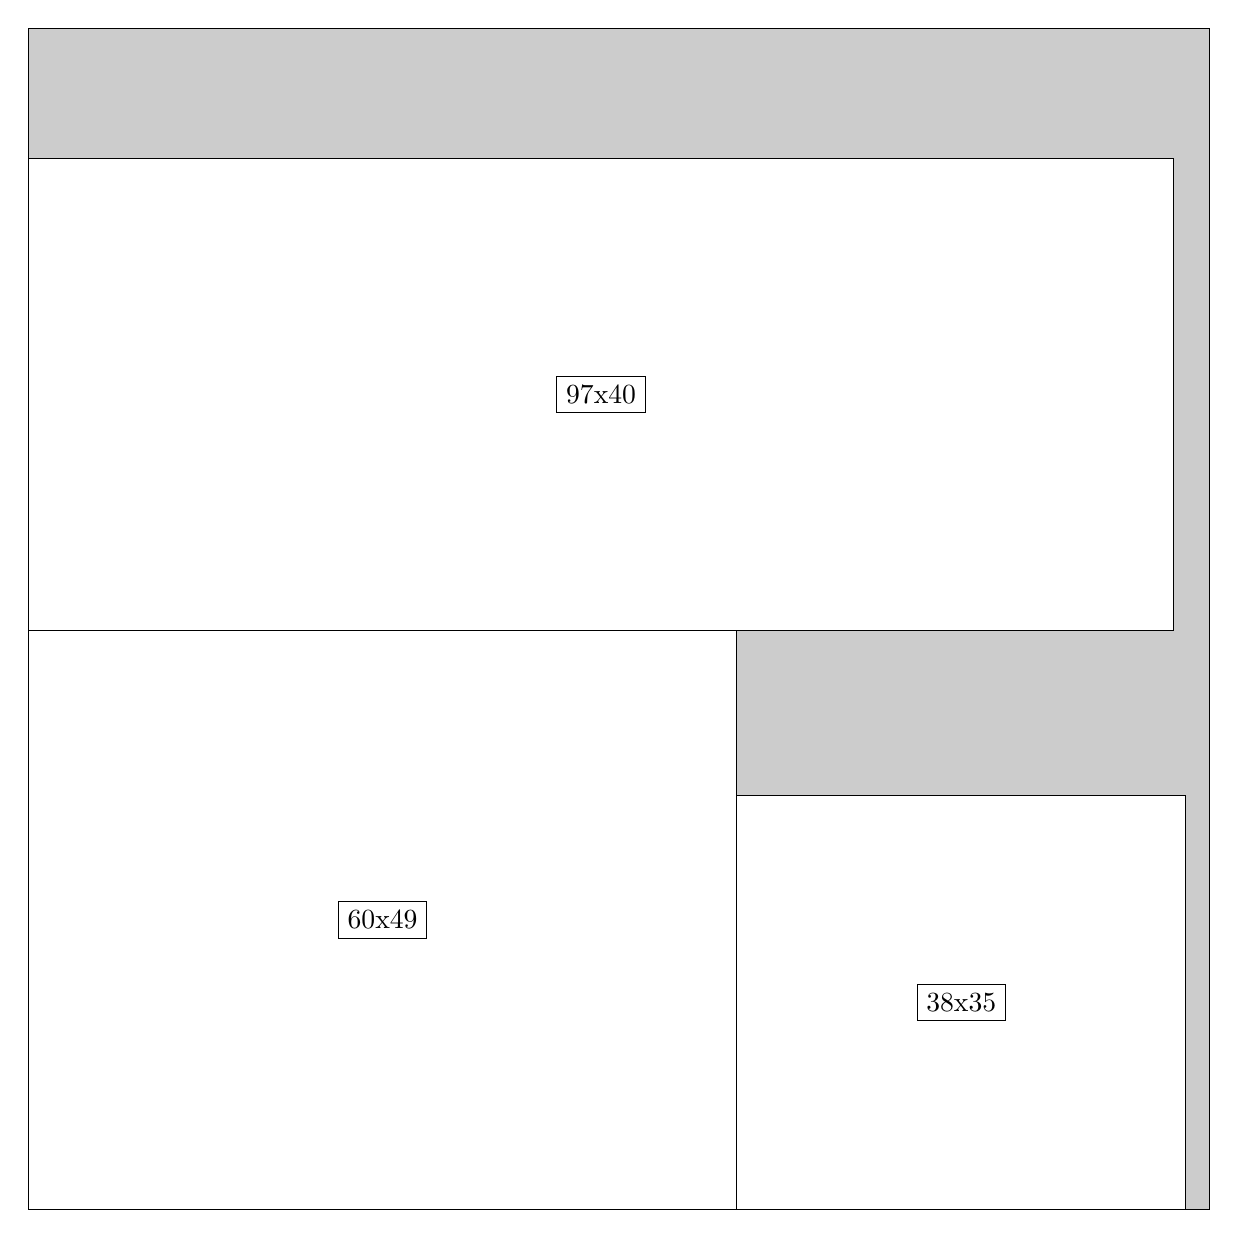
\begin{tikzpicture}[shorten >=1pt,scale=1.0,every node/.style={scale=1.0},->]
\tikzstyle{vertex}=[circle,fill=black!25,minimum size=14pt,inner sep=0pt]
\filldraw[fill=gray!40!white, draw=black] (0,0) rectangle (15.0,15.0);
\foreach \name/\x/\y/\w/\h in {97x40/0.0/7.35/14.549999999999999/6.0,60x49/0.0/0.0/9.0/7.35,38x35/9.0/0.0/5.7/5.25}
\filldraw[fill=white!40!white, draw=black] (\x,\y) rectangle node[draw] (\name) {\name} ++(\w,\h);
\end{tikzpicture}


w =97 , h =40 , x =0 , y =49 , v =3880
\par
w =60 , h =49 , x =0 , y =0 , v =2940
\par
w =38 , h =35 , x =60 , y =0 , v =1330
\par
\newpage


\end{document}